\documentclass[journal,onecolumn,12pt,a4paper]{IEEEtran}
\usepackage[T1]{fontenc}
\usepackage{mathptmx}
\usepackage{cite}
\usepackage{amsmath,amssymb}
\usepackage{graphicx}
\usepackage{booktabs}
\usepackage{tabularx}
\usepackage{adjustbox}
\usepackage{url}
\usepackage{algorithm}
\usepackage{algpseudocode}
\usepackage{balance}
\newcolumntype{Y}{>{\raggedright\arraybackslash}X}
\algnewcommand\algorithmicinput{\textbf{input:}}
\hyphenation{Lex-Front tokenizers}
\def\BibTeX{{\rm B\kern-.05em{\sc i\kern-.025em b}\kern-.08em T\kern-.1667em\lower.7ex\hbox{E}\kern-.125emX}}
\graphicspath{{../figures/vector/}}
\begin{document}
\title{LexFront: A Compiler-Style Lexer Used as a Pre-Tokenizer\\for Noisy English Text Classification}
\author{\IEEEauthorblockN{Veer Jahaan Arora (24BCB0080), Yash Aggarwal (24BKT0013),\\ and V C Pavitran (24BCE2019)}
\IEEEauthorblockA{School of Computer Science and Engineering (SCOPE), Vellore Institute of Technology (VIT), Vellore, India\\
Subject: Compiler Design Lab (BCSE307P) \quad Faculty: Suganthini C}}
\maketitle

\begin{abstract}
Text from social media is full of hashtags, mentions, links, emoticons and stretched-out words, and most tokenizers were not designed for it. We ask whether a lexical analyzer built the way a compiler builds one can do better. We built LexFront, a lexer with eleven token classes, longest-match scanning, error recovery, a symbol table and six switchable normalization rules, together with our own engine that turns regular expressions into an NFA, a DFA and a minimized DFA, checked against the PLY-based lexer that the experiments use. LexFront was compared with whitespace, NLTK and TweetTokenizer, and with BPE, WordPiece and Unigram subword tokenizers, with the classifier held fixed, on three core datasets, a collection of eight cleaned datasets, and four large datasets (Sentiment140, Civil Comments, Amazon polarity and Yelp). The result is consistent: LexFront is competitive but not better. With the tokenizer as the only change it stays within 0.00 to +0.46 accuracy points of NLTK on the large datasets, and it is clearly ahead only of whitespace splitting. It gives the lowest out-of-vocabulary rate and the smallest vocabulary among the word-level tokenizers. Most of the measured accuracy comes from the classifier and its tuning: moving from Naive Bayes to Logistic Regression is worth up to 17 points, and wider validated settings add 2 to 3 points. Subword tokenizers and a character n-gram baseline did not help. We report confidence intervals and the hypotheses that did not hold.
\end{abstract}

\begin{IEEEkeywords}
lexical analysis, DFA, tokenization, noisy text, text classification, subword tokenization
\end{IEEEkeywords}

\section{Introduction}\label{sec:1}
A lot of the text we want to classify today comes from social media, and it is messy. People write hashtags, @-mentions, links and emoticons in the middle of sentences, they stretch words out (``soooo good''), and they use slang that no dictionary has. A tokenizer that was built for clean newspaper text can split these things in awkward ways, and since a classifier only sees the tokens, a bad split can cost accuracy. This problem has been known for a while, and early work on tweets already treated tokenization and normalization as problems of their own \cite{r2}, \cite{r3}.

Compilers face a very similar problem in their first phase. A lexical analyzer reads a stream of characters and groups them into tokens, using regular expressions, a longest-match rule, a symbol table and some way of recovering from characters it cannot match \cite{r1}. That is close to what a tweet tokenizer has to do, so we wanted to see how far the compiler approach carries over. Our idea was to build a lexer in the compiler-design style, use it as a pre-tokenizer for text classification, and compare it with existing tokenizers while keeping everything else in the pipeline fixed. The question we try to answer is whether a compiler-style lexer classifies noisy text better than the tokenizers people already use.

The work in this report makes four contributions. First, we built LexFront, a lexer with a priority-ordered token specification, a normalizer and a symbol table, together with our own regex-to-DFA engine that implements Thompson construction, subset construction and Moore minimization. Second, we set up a controlled comparison in which the tokenizer is the only thing that changes, with confidence intervals and significance tests so that small differences are not over-read. Third, we ran ablations that switch each normalization rule off separately, and a subword extension that combines LexFront with BPE and compares it with WordPiece and Unigram \cite{r4}. Fourth, we checked how far the results hold up with a fair tuning protocol, a collection of eight cleaned datasets, and four large datasets with hypotheses written down before the runs. Section~\ref{sec:2} reviews the literature, Section~\ref{sec:3} describes the proposed system and its five modules, Section~\ref{sec:4} gives the implementation and results, Section~\ref{sec:5} compares performance, and Section~\ref{sec:6} concludes.

\section{Literature Survey}\label{sec:2}
We grouped the related work into five areas: compiler front ends and automata, tokenization of noisy text, subword tokenization, text classification baselines, and evaluation methodology. Each subsection ends with a short note on how it connects to our work.

\subsection{Compiler front ends and finite automata}\label{sec:2.1}
The standard reference for the first phase of a compiler is the textbook by Aho, Lam, Sethi and Ullman \cite{r1}, which describes how a lexical analyzer turns regular expressions into a recognizer and how a symbol table and error recovery fit around it. The construction we implement goes back to Thompson \cite{r5}, who showed how to build a nondeterministic automaton from a regular expression piece by piece. The subset construction that converts it to a deterministic automaton, and the closure properties that make this possible, are covered in the automata theory text by Hopcroft, Motwani and Ullman \cite{r6}. For minimization we followed the partition-refinement idea that goes back to Moore \cite{r7}.

On the practical side, Lex \cite{r8} generated scanners from regular expressions and was designed to work together with the parser generator Yacc \cite{r9}. PLY \cite{r10} brings the same style to Python, and the tokenizer used in our experiments is built on it. All of these tools take a list of patterns in priority order and apply longest match, with ties going to the earlier rule, which is the behaviour we copied. What we take from this area is the whole design vocabulary of LexFront: token classes, longest match, priority, semantic actions on tokens and panic-mode error recovery.

\subsection{Tokenization and normalization of noisy text}\label{sec:2.2}
Gimpel et al. \cite{r2} built a part-of-speech tagger specifically for Twitter and had to deal with hashtags, mentions, URLs and emoticons as tokens in their own right, and Owoputi et al. \cite{r11} improved it further with word clusters. Han and Baldwin \cite{r3} looked at the other side of the problem and studied how to normalize the ill-formed words in short text messages into their standard forms. Later, the shared tasks at the Workshop on Noisy User-generated Text made lexical normalization a regular benchmark \cite{r12}. These papers show that for noisy text the choice of what counts as a token, and what is done to it afterwards, is an open design decision and not a solved detail.

Most practical systems use general toolkits. NLTK \cite{r13} ships a standard word tokenizer and a TweetTokenizer that handles emoticons, handles and elongation, and these are the two existing tokenizers we compare against. Textbooks on information retrieval also treat tokenization as a step with real consequences for what ends up in the index \cite{r14}. Large language models for tweets follow a similar pattern. BERTweet \cite{r15}, which was pre-trained on English tweets, normalizes user mentions and links before tokenization, which is close in spirit to the placeholders in our normalizer.

\subsection{Subword tokenization}\label{sec:2.3}
Subword methods avoid the unknown-word problem by splitting rare words into smaller pieces. Sennrich et al. \cite{r4} adapted byte pair encoding (BPE) for neural machine translation, and the WordPiece model, first described for Japanese and Korean voice search \cite{r16}, was used in Google's translation system \cite{r17}. Kudo \cite{r18} proposed a unigram language model for subword segmentation and the SentencePiece toolkit \cite{r19} packaged BPE and unigram tokenization in a language-independent way. BERT \cite{r20} uses a WordPiece vocabulary and RoBERTa \cite{r21} uses byte-level BPE, so these methods sit under most modern language models.

Several papers question whether these tokenizers are optimal. Bostrom and Durrett \cite{r22} argue that BPE is suboptimal for language model pretraining and that a unigram-based tokenizer can do better. Rust et al. \cite{r23} show that the quality of the tokenizer affects how well multilingual models perform on single languages, and Toraman et al. \cite{r24} study how tokenization choices affect language models for Turkish. Mielke et al. \cite{r25} give a broad survey of tokenization and open-vocabulary modeling. Bojanowski et al. \cite{r26} used character n-gram subwords to enrich word vectors, which is another way of handling rare and misspelled words. Almost all of this work targets neural models trained at large scale. Our setting is smaller and uses a linear classifier, so we do not expect the same conclusions, and we treat the subword results as a separate question.

\subsection{Text classification baselines and representations}\label{sec:2.4}
Multinomial Naive Bayes is a classic text classifier and has been compared closely with other event models by McCallum and Nigam \cite{r27}. Wang and Manning \cite{r28} showed that simple Naive Bayes-style models with bigrams are strong baselines for sentiment and topic classification, and Joulin et al. \cite{r29} made a similar point with fastText, which is a fast linear classifier. Features for such classifiers are usually built with TF-IDF, which combines the idea of inverse document frequency \cite{r30} with term weighting schemes studied by Salton and Buckley \cite{r31}. Dense representations such as word2vec \cite{r32} and GloVe \cite{r33}, and later the Transformer \cite{r34}, moved the field toward neural models, but linear models on TF-IDF features remain a common and transparent baseline. We use scikit-learn \cite{r35} for TF-IDF, Naive Bayes and Logistic Regression.

We deliberately kept to this baseline setting. A linear model on TF-IDF features is sensitive to exactly the thing we want to study, which is how the text is split into tokens, and it is cheap enough to run the whole grid of tokenizers on full datasets.

\subsection{Evaluation and statistical testing}\label{sec:2.5}
Many papers report a difference of a few tenths of a point without saying whether it is bigger than the noise. The bootstrap \cite{r36} gives a way to put confidence intervals on a metric by resampling the test set, and McNemar's test \cite{r37} compares two classifiers on the same test examples, which is the paired case we have. Dietterich \cite{r38} discussed which tests are appropriate for comparing classifiers, and Dror et al. \cite{r39} wrote a guide to significance testing for NLP. We follow these ideas: paired bootstrap intervals and McNemar's test for every tokenizer difference, and a note on what the intervals do and do not cover.

\subsection{Gap addressed by this work}\label{sec:2.6}
From the survey we see plenty of work on tokenizers for neural models and on normalization for tweets, and a long tradition of lexer construction in compilers. What we did not find is a controlled comparison that takes a lexer built with standard compiler machinery and puts it next to existing tokenizers with the classifier held fixed. LexFront and the experiments in this report try to fill that gap on a small scale, and we try to be careful about what the results do and do not show.

\section{Proposed System}\label{sec:3}
\subsection{Overview}\label{sec:3.1}
The system is a text classification pipeline in which the tokenizer is the part we swap. Raw text goes into one of the tokenizers, the tokens are turned into TF-IDF features, and a classifier (Naive Bayes or Logistic Regression) predicts the label. Because everything after the tokenizer is identical, any difference in the results can be put down to the tokenizer and not to the rest of the pipeline. Around that pipeline we have an evaluation layer that computes accuracy, macro-F1, confidence intervals, significance tests and a few intrinsic measures such as out-of-vocabulary rate and vocabulary size.

We organised the work into five modules. Module 1 is the existing methodology that serves as the baseline. Module 2 is the LexFront lexer and the DFA engine. Module 3 is the normalizer and symbol table together with the ablation of its rules. Module 4 is the subword stage, which includes the LexFront + BPE hybrid and the comparison with WordPiece and Unigram. Module 5 is the protocol for tuning, scale and robustness: fair classifier tuning, larger datasets, and a noise test. Modules 2, 3, 4 and 5 are the new contribution, and we give pseudocode for each of them.

\subsection{Architecture diagram}\label{sec:3.2}
\begin{figure}[!t]
\centering
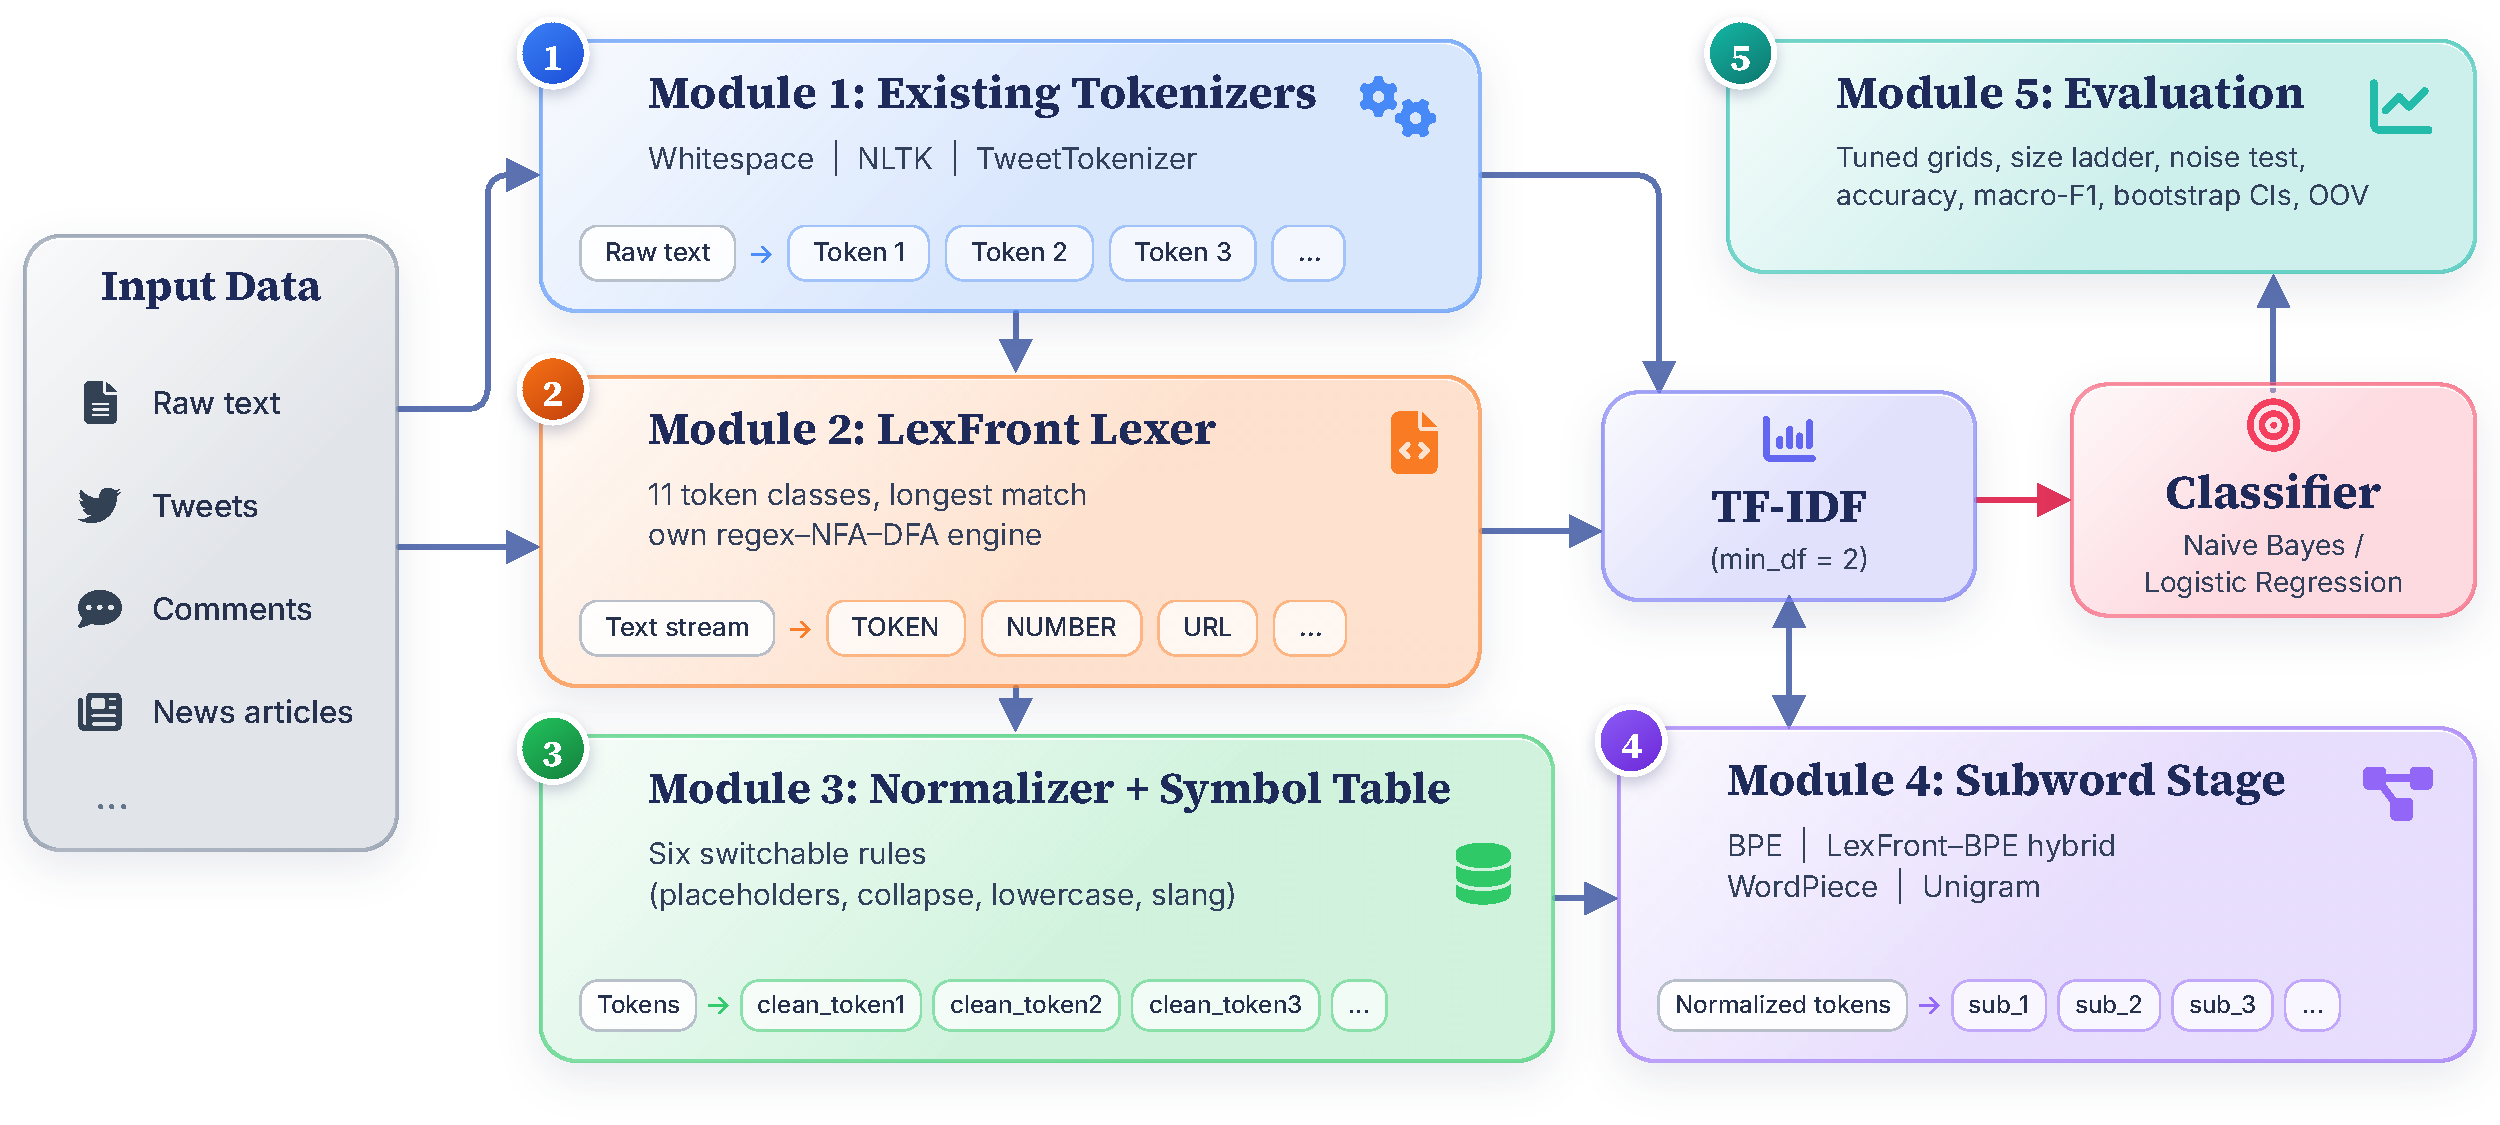
\includegraphics[width=0.96\columnwidth]{architecture}
\caption{Architecture of the proposed system and its five modules}\label{fig:1}
\end{figure}

\subsection{Module 1: Existing methodology (baseline)}\label{sec:3.3}
Module 1 holds the setup that LexFront is compared against. It has three existing tokenizers, which are whitespace splitting, the NLTK word tokenizer and NLTK's TweetTokenizer \cite{r13}. Their tokens go into TF-IDF with min\_df=2, and the features go into a majority-class baseline, Multinomial Naive Bayes (the existing method) and Logistic Regression with max\_iter=1000 and seed 0. All fits run on a single thread, because we saw that the BLAS thread count changed some Logistic Regression metrics in the last digits. Every run writes a JSON file with its configuration, a fingerprint and the metrics, and stores its test predictions so that the confidence intervals can be computed without refitting.

The evaluation loop shared by all modules is short, and we give it as Algorithm~\ref{alg:1} below.

\begin{algorithm}[!t]
\footnotesize
\caption{Evaluation loop shared by all modules}\label{alg:1}
\begin{algorithmic}[1]
\State \textbf{for} dataset \textbf{in} [tweet\_topic, go\_emotions, ag\_news]:
\State \hspace*{1.0em}train, test $\leftarrow$ load(dataset)
\State \hspace*{1.0em}\textbf{for} tokenizer \textbf{in} tokenizer\_list:
\State \hspace*{2.0em}X\_train $\leftarrow$ TfidfVectorizer(tokenizer, min\_df=2).fit\_transform(train)
\State \hspace*{2.0em}X\_test  $\leftarrow$ vectorizer.transform(test)
\State \hspace*{2.0em}\textbf{for} clf \textbf{in} [majority, naive\_bayes, logistic\_regression]:
\State \hspace*{3.0em}clf.fit(X\_train, y\_train)
\State \hspace*{3.0em}record $\leftarrow$ \{config, accuracy, macro\_f1, timings, versions\}
\State \hspace*{3.0em}save record (with config + code fingerprint) and test predictions
\State tables, figures and statistics are built only from the saved files
\end{algorithmic}
\end{algorithm}

\subsection{Module 2: LexFront lexer and DFA engine}\label{sec:3.4}
This is the main new module. LexFront defines eleven token classes in priority order (in \texttt{lexer/\allowbreak{}token\_\allowbreak{}spec.py}): URL, MENTION, HASHTAG, EMOTICON, EMOJI, NUMBER, CONTRACTION, ELONGATED, WORD, PUNCT, and UNKNOWN as the fallback. A PLY-based scanner takes the longest match at each position, ties go to the earlier class, and a character that matches nothing becomes an UNKNOWN token so scanning continues, which is panic-mode recovery.

Our own regex-to-DFA engine and its table-driven scanner are given as Algorithms~\ref{alg:2} and~\ref{alg:3}, shown side by side: Algorithm~\ref{alg:2} builds the automaton and Algorithm~\ref{alg:3} scans with it.

\begin{figure}[!t]
\centering
\begin{minipage}[t]{0.485\textwidth}
\hrule\vspace{2pt}\scriptsize\refstepcounter{algorithm}\label{alg:2}\textbf{Algorithm 2} Regex to minimized DFA\vspace{2pt}\hrule\vspace{1pt}
\begin{algorithmic}[1]
\State \hspace*{1.0em}\textbf{input} : rules [(name\_i, regex\_i)], \textbf{in} priority order
\State \hspace*{1.0em}asts  $\leftarrow$ [parse(regex\_i) \textbf{for} each rule]
\State \hspace*{1.0em}atoms $\leftarrow$ alphabet split at every range boundary
\State \hspace*{1.0em}NFA   $\leftarrow$ new start state
\State \hspace*{1.0em}\textbf{for} i, ast \textbf{in} asts:
\State \hspace*{2.0em}(s, t) $\leftarrow$ thompson(ast)
\State \hspace*{2.0em}add eps-edge NFA.start $\rightarrow$ s ; accepting[t] $\leftarrow$ i
\State \hspace*{1.0em}S0 $\leftarrow$ eps\_closure(\{NFA.start\}) ; DFA.states $\leftarrow$ \{S0\}
\State \hspace*{1.0em}\textbf{while} worklist \textbf{not} empty:
\State \hspace*{2.0em}S $\leftarrow$ pop(worklist)
\State \hspace*{2.0em}\textbf{for} each atom a:
\State \hspace*{3.0em}T $\leftarrow$ eps\_closure(move(S, a))
\State \hspace*{3.0em}\textbf{if} T \textbf{not} empty: add T \textbf{if} new ; trans[S][a] $\leftarrow$ T
\State \hspace*{1.0em}\textbf{for} each DFA state S:
\State \hspace*{2.0em}S.accepts $\leftarrow$ min accepting[q], q \textbf{in} S
\Statex \hspace*{1.0em}{\scriptsize$\triangleright$ \textit{Moore minimization}}
\State \hspace*{1.0em}block[S] $\leftarrow$ id of S.accepts
\State \hspace*{1.0em}\textbf{repeat}:
\State \hspace*{2.0em}sig[S] $\leftarrow$ (block[S], block of each target)
\State \hspace*{2.0em}block[S] $\leftarrow$ id of sig[S]
\State \hspace*{1.0em}\textbf{until} the number of blocks stops growing
\State \hspace*{1.0em}merge states with equal block
\end{algorithmic}
\hrule
\end{minipage}
\hfill
\begin{minipage}[t]{0.485\textwidth}
\hrule\vspace{2pt}\scriptsize\refstepcounter{algorithm}\label{alg:3}\textbf{Algorithm 3} Longest-match scanner with error recovery\vspace{2pt}\hrule\vspace{1pt}
\begin{algorithmic}[1]
\State \hspace*{1.0em}pos $\leftarrow$ 0
\State \hspace*{1.0em}\textbf{while} pos \textless{} len(text):
\State \hspace*{2.0em}\textbf{if} text[pos] is whitespace: pos++ ; \textbf{continue}
\State \hspace*{2.0em}state $\leftarrow$ start ; last $\leftarrow$ none ; i $\leftarrow$ pos
\State \hspace*{2.0em}\textbf{while} i \textless{} len(text):
\State \hspace*{3.0em}state $\leftarrow$ table[state][atom\_of(text[i])]
\State \hspace*{3.0em}\textbf{if} state == DEAD: \textbf{break}
\State \hspace*{3.0em}i++
\State \hspace*{3.0em}\textbf{if} accepts[state] is \textbf{not} none:
\State \hspace*{4.0em}last $\leftarrow$ (i, accepts[state])
\State \hspace*{2.0em}\textbf{if} last is none: \hfill{\scriptsize$\triangleright$ \textit{error recovery}}
\State \hspace*{3.0em}emit (UNKNOWN, text[pos]) ; pos++
\State \hspace*{2.0em}\textbf{else}:
\State \hspace*{3.0em}emit (class[rule], text[pos:end]) ; pos $\leftarrow$ end
\end{algorithmic}
\hrule
\end{minipage}
\end{figure}

Besides the PLY lexer we wrote our own engine in \texttt{lexer/\allowbreak{}dfa/\allowbreak{}}. A recursive-descent parser turns each regular expression into an AST, Thompson construction \cite{r5} gives an NFA, subset construction \cite{r6} gives a DFA over an alphabet that is split into atoms, and Moore's partition refinement \cite{r7} minimizes it. The engine covers four classes (EMOTICON, HASHTAG, MENTION and WORD). The tokenizer used in the experiments is the PLY-based one, and our engine is a separate implementation that a test checks against it: it produces the same tokens on those four classes. ELONGATED is not part of the engine because its usual regex, (.)\textbackslash{}1\{2,\}, needs a back-reference, which regular expressions cannot express.

\subsection{Module 3: Normalizer, symbol table and rule ablation}\label{sec:3.5}
After a token has been scanned, a semantic action maps it to its canonical form, much like the action block attached to a Lex rule. LexFront has six such rules in \texttt{lexer/\allowbreak{}normalize.py}, and each one can be switched on or off by itself. URLs become \textless{}URL\textgreater{}, mentions become \textless{}USER\textgreater{} and numbers become \textless{}NUM\textgreater{}. Runs of three or more identical letters are shortened to two (``sooooo'' becomes ``soo''). Word-like tokens are lowercased, and a lookup in a slang table of 30 entries expands things like ``u'' into ``you''. The symbol table stores an id, a frequency and a class for each token.

Because every rule has its own switch, we can run an ablation in which one rule is removed at a time, and a case-sensitivity check in which TF-IDF's own lowercasing is turned off. That is how we find out which rules actually help. Pseudocode for the normalizer follows.

\begin{algorithm}[!t]
\footnotesize
\caption{Token normalization, tokenization and rule ablation}\label{alg:4}
\begin{algorithmic}[1]
\State normalize\_token(cls, lexeme, config):
\State \hspace*{1.0em}\textbf{if} cls == URL     and config.url:      \textbf{return} ["\textless{}URL\textgreater{}"]
\State \hspace*{1.0em}\textbf{if} cls == MENTION and config.mention:  \textbf{return} ["\textless{}USER\textgreater{}"]
\State \hspace*{1.0em}\textbf{if} cls == NUMBER  and config.number:   \textbf{return} ["\textless{}NUM\textgreater{}"]
\State \hspace*{1.0em}\textbf{if} cls \textbf{not} \textbf{in} \{WORD, CONTRACTION, ELONGATED\}: \textbf{return} [lexeme]
\State \hspace*{1.0em}\textbf{if} cls == ELONGATED and config.elongated:
\State \hspace*{2.0em}lexeme $\leftarrow$ shorten every run of 3+ identical letters to 2
\State \hspace*{1.0em}\textbf{if} config.lowercase:  lexeme $\leftarrow$ lowercase(lexeme)
\State \hspace*{1.0em}\textbf{if} config.slang and lexeme \textbf{in} slang\_table:
\State \hspace*{2.0em}\textbf{return} split(slang\_table[lexeme]) \hfill{\scriptsize$\triangleright$ \textit{may be several words}}
\State \hspace*{1.0em}\textbf{return} [lexeme]
\State tokenize(text):
\State \hspace*{1.0em}\textbf{for} (cls, lexeme) \textbf{in} scan(text):
\State \hspace*{2.0em}\textbf{for} form \textbf{in} normalize\_token(cls, lexeme, config):
\State \hspace*{3.0em}symbol\_table.update(form, cls) \hfill{\scriptsize$\triangleright$ \textit{id, frequency, class}}
\State \hspace*{3.0em}emit form
\State ablation: \textbf{for} rule \textbf{in} [url, mention, number, elongated,
\State \hspace*{6.0em}lowercase, slang, all]:
\State \hspace*{3.0em}run the full pipeline with that rule switched off
\end{algorithmic}
\end{algorithm}

\subsection{Module 4: Subword stage and the LexFront + BPE hybrid}\label{sec:3.6}
Module 4 adds learned vocabularies on top of, and next to, the word-level tokenizers. We trained BPE, WordPiece and Unigram models with the Hugging Face tokenizers library on the training split only, lowercased, with a vocabulary of 8000 pieces (BPE was also run at 32000). Pieces that continue a word carry the \#\# marker in BPE and WordPiece. We also built a two-stage hybrid that follows the compiler idea of passing different token types to different handlers. LexFront decides the class of each token first. Structural tokens such as placeholders, hashtags, emoticons, emoji, punctuation and error tokens are passed through whole, and only the word-like tokens are handed to a BPE model that was trained on the word-like tokens of the training texts.

Making the training deterministic took some care. The trainer assigns ids to the \#\# alphabet in hash-map order, so two trainings on the same text could merge in a different order. We fixed this by passing a sorted alphabet as special tokens and removing them from the added-token list afterwards. We also checked that texts from the test split do not leak into the trained vocabularies. The hybrid is described in the pseudocode below.

\begin{algorithm}[!t]
\footnotesize
\caption{LexFront + BPE hybrid tokenizer}\label{alg:5}
\begin{algorithmic}[1]
\State train\_hybrid(train\_texts):
\State \hspace*{1.0em}words $\leftarrow$ []
\State \hspace*{1.0em}\textbf{for} text \textbf{in} train\_texts:
\State \hspace*{2.0em}\textbf{for} (cls, lexeme, forms) \textbf{in} LexFront.analyze(lowercase(text)):
\State \hspace*{3.0em}\textbf{if} cls \textbf{in} \{WORD, CONTRACTION, ELONGATED\}: words.extend(forms)
\State \hspace*{1.0em}BPE $\leftarrow$ train\_bpe(join(words), vocab\_size, sorted\_alphabet)
\State tokenize\_hybrid(text):
\State \hspace*{1.0em}out $\leftarrow$ []
\State \hspace*{1.0em}\textbf{for} (cls, lexeme, forms) \textbf{in} LexFront.analyze(text):
\State \hspace*{2.0em}\textbf{for} form \textbf{in} forms:
\State \hspace*{3.0em}\textbf{if} cls \textbf{in} \{WORD, CONTRACTION, ELONGATED\}:
\State \hspace*{4.0em}out.extend(BPE.encode(form))
\State \hspace*{3.0em}\textbf{else}:
\State \hspace*{4.0em}out.append(form) \hfill{\scriptsize$\triangleright$ \textit{structural: pass through}}
\State \hspace*{1.0em}\textbf{return} out
\end{algorithmic}
\end{algorithm}

\subsection{Module 5: Tuning, scale and robustness protocol}\label{sec:3.7}
Module 5 is about how far the results of Modules 1 to 4 can be trusted. It has three parts. The first is a fair tuning protocol. For every tokenizer we choose the TF-IDF settings (word n-grams up to length 3, plain or sublinear term frequency, minimum document frequency 2 or 5) and the classifier parameter (C from 0.3 to 30 for Logistic Regression, alpha from 0.03 to 1 for Naive Bayes) on a validation slice taken from the training data only. The grid is the same for every tokenizer, and the test set is scored once at the end. This matters because a tokenizer comparison at default settings can simply favour whichever tokenizer happens to suit those defaults.

The second part is scale. We cleaned each dataset with fixed rules (empty texts, texts with conflicting labels, duplicates, and test texts that also occur in the training set) and, for Sentiment140, we split by user so that no user appears in both train and test. On Sentiment140 we also ran a size ladder from 10,000 to the full training set. The third part is a noise test: seeded synthetic noise is added to the test text only (a light level, where 10\% of the eligible words are corrupted, and a heavy level with 30\%), to see which tokenizer loses less accuracy. Hypotheses and a practical margin of plus or minus 0.5 points were written down before the runs in protocol documents (\path{docs/LARGE_PROTOCOL.md}, \path{docs/BOOST_PROTOCOL.md} and \path{docs/D_PROTOCOL.md}). Each difference is then reported as within, beyond or unclear relative to that margin. Algorithm~\ref{alg:6} below summarizes the tuning and comparison steps.

\begin{algorithm}[!t]
\footnotesize
\caption{Tuning, paired comparison and noise test}\label{alg:6}
\begin{algorithmic}[1]
\State tune\_and\_test(tokenizer, classifier, train, test):
\State \hspace*{1.0em}fit, val $\leftarrow$ stratified split of train (at most 100,000 / 20,000 examples)
\State \hspace*{1.0em}best $\leftarrow$ none
\State \hspace*{1.0em}\textbf{for} vectorizer \textbf{in} VECTORIZER\_GRID: \hfill{\scriptsize$\triangleright$ \textit{word n-grams, raw or sublinear tf, min\_df}}
\State \hspace*{2.0em}X\_fit $\leftarrow$ vectorizer.fit\_transform(tokenizer(fit))
\State \hspace*{2.0em}X\_val $\leftarrow$ vectorizer.transform(tokenizer(val))
\State \hspace*{2.0em}\textbf{for} value \textbf{in} PARAMETER\_GRID[classifier]: \hfill{\scriptsize$\triangleright$ \textit{C or alpha}}
\State \hspace*{3.0em}score $\leftarrow$ accuracy(model(value).fit(X\_fit, y\_fit).predict(X\_val), y\_val)
\State \hspace*{3.0em}keep the best (vectorizer, value)
\State \hspace*{1.0em}refit the best setting on the full training set
\State \hspace*{1.0em}score the test set once, save predictions
\Statex \hspace*{1.0em}{\scriptsize$\triangleright$ \textit{the same grids are used for every tokenizer}}
\State compare(A, B): \hfill{\scriptsize$\triangleright$ \textit{same test examples}}
\State \hspace*{1.0em}diff $\leftarrow$ accuracy(A) - accuracy(B)
\State \hspace*{1.0em}CI   $\leftarrow$ percentile bootstrap of diff over the test examples
\State \hspace*{1.0em}verdict $\leftarrow$ within | beyond | unclear   against the +-0.5 point margin
\State noise\_test(tokenizer): add seeded noise to the test text only; accuracy lost = clean - noisy
\end{algorithmic}
\end{algorithm}

\section{Results and Implementation}\label{sec:4}
The system is written in Python and every number below was read from the JSON result files in the repository, which are written by the scripts we ran. The core datasets use full data with no subsampling. For Civil Comments and Amazon polarity we took a seeded random sample of about 500,000 training examples, for Yelp 300,000 training and 50,000 test examples, and Sentiment140 is used in full after cleaning. Each cell is a single training run. The 95\% confidence intervals are paired percentile bootstraps over the test examples, with McNemar's test for accuracy on the core datasets. They cover the draw of the test set, not training randomness.

\subsection{Dataset description}\label{sec:4.1}
We used English datasets that differ in style and size, in three groups. The core group has three datasets used in Modules 1 to 4: tweet\_topic \cite{r40} has tweets labelled with six topics, go\_emotions \cite{r41} has Reddit comments labelled with 28 emotion classes (we kept only the single-label examples), and ag\_news \cite{r42} has news articles in four categories. The first two are noisy and informal, while ag\_news is relatively clean, which gives a useful contrast. The collection group adds five tweet\_eval tasks (sentiment, emotion, irony, hate and offensive language), so that together with the core datasets there are eight cleaned datasets. The large group has Sentiment140 (1.6 million tweets, split by user), Civil Comments (comments with a toxicity label, where the toxic class is rare), Amazon polarity (product reviews) and Yelp (reviews with five star classes, which tests a many-class problem). Table~\ref{tab:1} lists the core and large datasets, and the last column is the share of the largest class in the test set, which is also the accuracy of the majority baseline. For the large datasets the sizes are after cleaning and, for Civil Comments and Amazon polarity, after taking a seeded random sample of about 500,000 training examples (300,000 training and 50,000 test examples for Yelp).

\begin{table}[!tb]
\caption{Datasets used}\label{tab:1}
\centering
\footnotesize
\setlength{\tabcolsep}{4pt}
\begin{tabular}{llllll}
\toprule
\textbf{Dataset} & \textbf{Source} & \textbf{Train docs} & \textbf{Test docs} & \textbf{Labels} & \textbf{Largest test class \%} \\
\midrule
tweet\_topic & \path{cardiffnlp/tweet_topic_single} & 3,598 & 3,399 & 6 & 40.01 \\
go\_emotions & go\_emotions (simplified) & 36,308 & 4,590 & 28 & 34.99 \\
ag\_news & \path{fancyzhx/ag_news} & 120,000 & 7,600 & 4 & 25.00 \\
Sentiment140 & \path{bdanko/sentiment140} & 1,495,821 & 78,278 & 2 & 50.28 \\
Civil Comments & \path{google/civil_comments} & 495,469 & 95,942 & 2 (toxic is rare) & 92.02 \\
Amazon polarity & \path{fancyzhx/amazon_polarity} & 499,993 & 99,996 & 2 & 50.04 \\
Yelp reviews & \path{Yelp/yelp_review_full} & 299,979 & 49,994 & 5 & 20.00 \\
\bottomrule
\end{tabular}
\end{table}

\subsection{Module 1: existing tokenizers}\label{sec:4.2}
Table~\ref{tab:2} gives accuracy and macro-F1 for the three existing tokenizers with each classifier. The first thing we notice is how little the tokenizer matters compared with the classifier. On go\_emotions, switching from Naive Bayes to Logistic Regression is worth around 17 points for every tokenizer, while the spread between tokenizers under Logistic Regression is about 2 points. NLTK and TweetTokenizer are slightly ahead of plain whitespace splitting in nearly every row. Naive Bayes on go\_emotions is close to the majority baseline in accuracy, and its macro-F1 is very low, which means it mostly predicts the large classes.

\subsection{Module 2: LexFront lexer and DFA engine}\label{sec:4.3}
\par\noindent\textit{Automaton sizes.}
Table~\ref{tab:3} shows how big each automaton is. The four classes are small. The combined automaton goes from 43 NFA states to 12 DFA states, and minimization brings it down to 10. WORD shrinks from 3 DFA states to 2 and EMOTICON from 6 to 5, so minimization does remove real redundancy. We also compiled ELONGATED by spelling it out as 26 separate branches, only to see what happens. It is not part of LexFront, but it shows how fast the construction can grow, from 221 NFA states to 157 DFA states and 54 after minimization.

\begin{table}[!tb]
\caption{Automaton sizes}\label{tab:3}
\centering
\footnotesize
\setlength{\tabcolsep}{4pt}
\begin{tabular}{lllll}
\toprule
\textbf{Automaton} & \textbf{Alphabet atoms} & \textbf{NFA states} & \textbf{DFA states} & \textbf{Minimized DFA states} \\
\midrule
MENTION & 5 & 9 & 3 & 3 \\
HASHTAG & 8 & 9 & 3 & 3 \\
EMOTICON & 17 & 19 & 6 & 5 \\
WORD & 6 & 9 & 3 & 2 \\
Combined (4 classes) & 31 & 43 & 12 & 10 \\
ELONGATED, 26 branches (extra) & 26 & 221 & 157 & 54 \\
\bottomrule
\end{tabular}
\end{table}

\begin{figure}[!t]
\centering
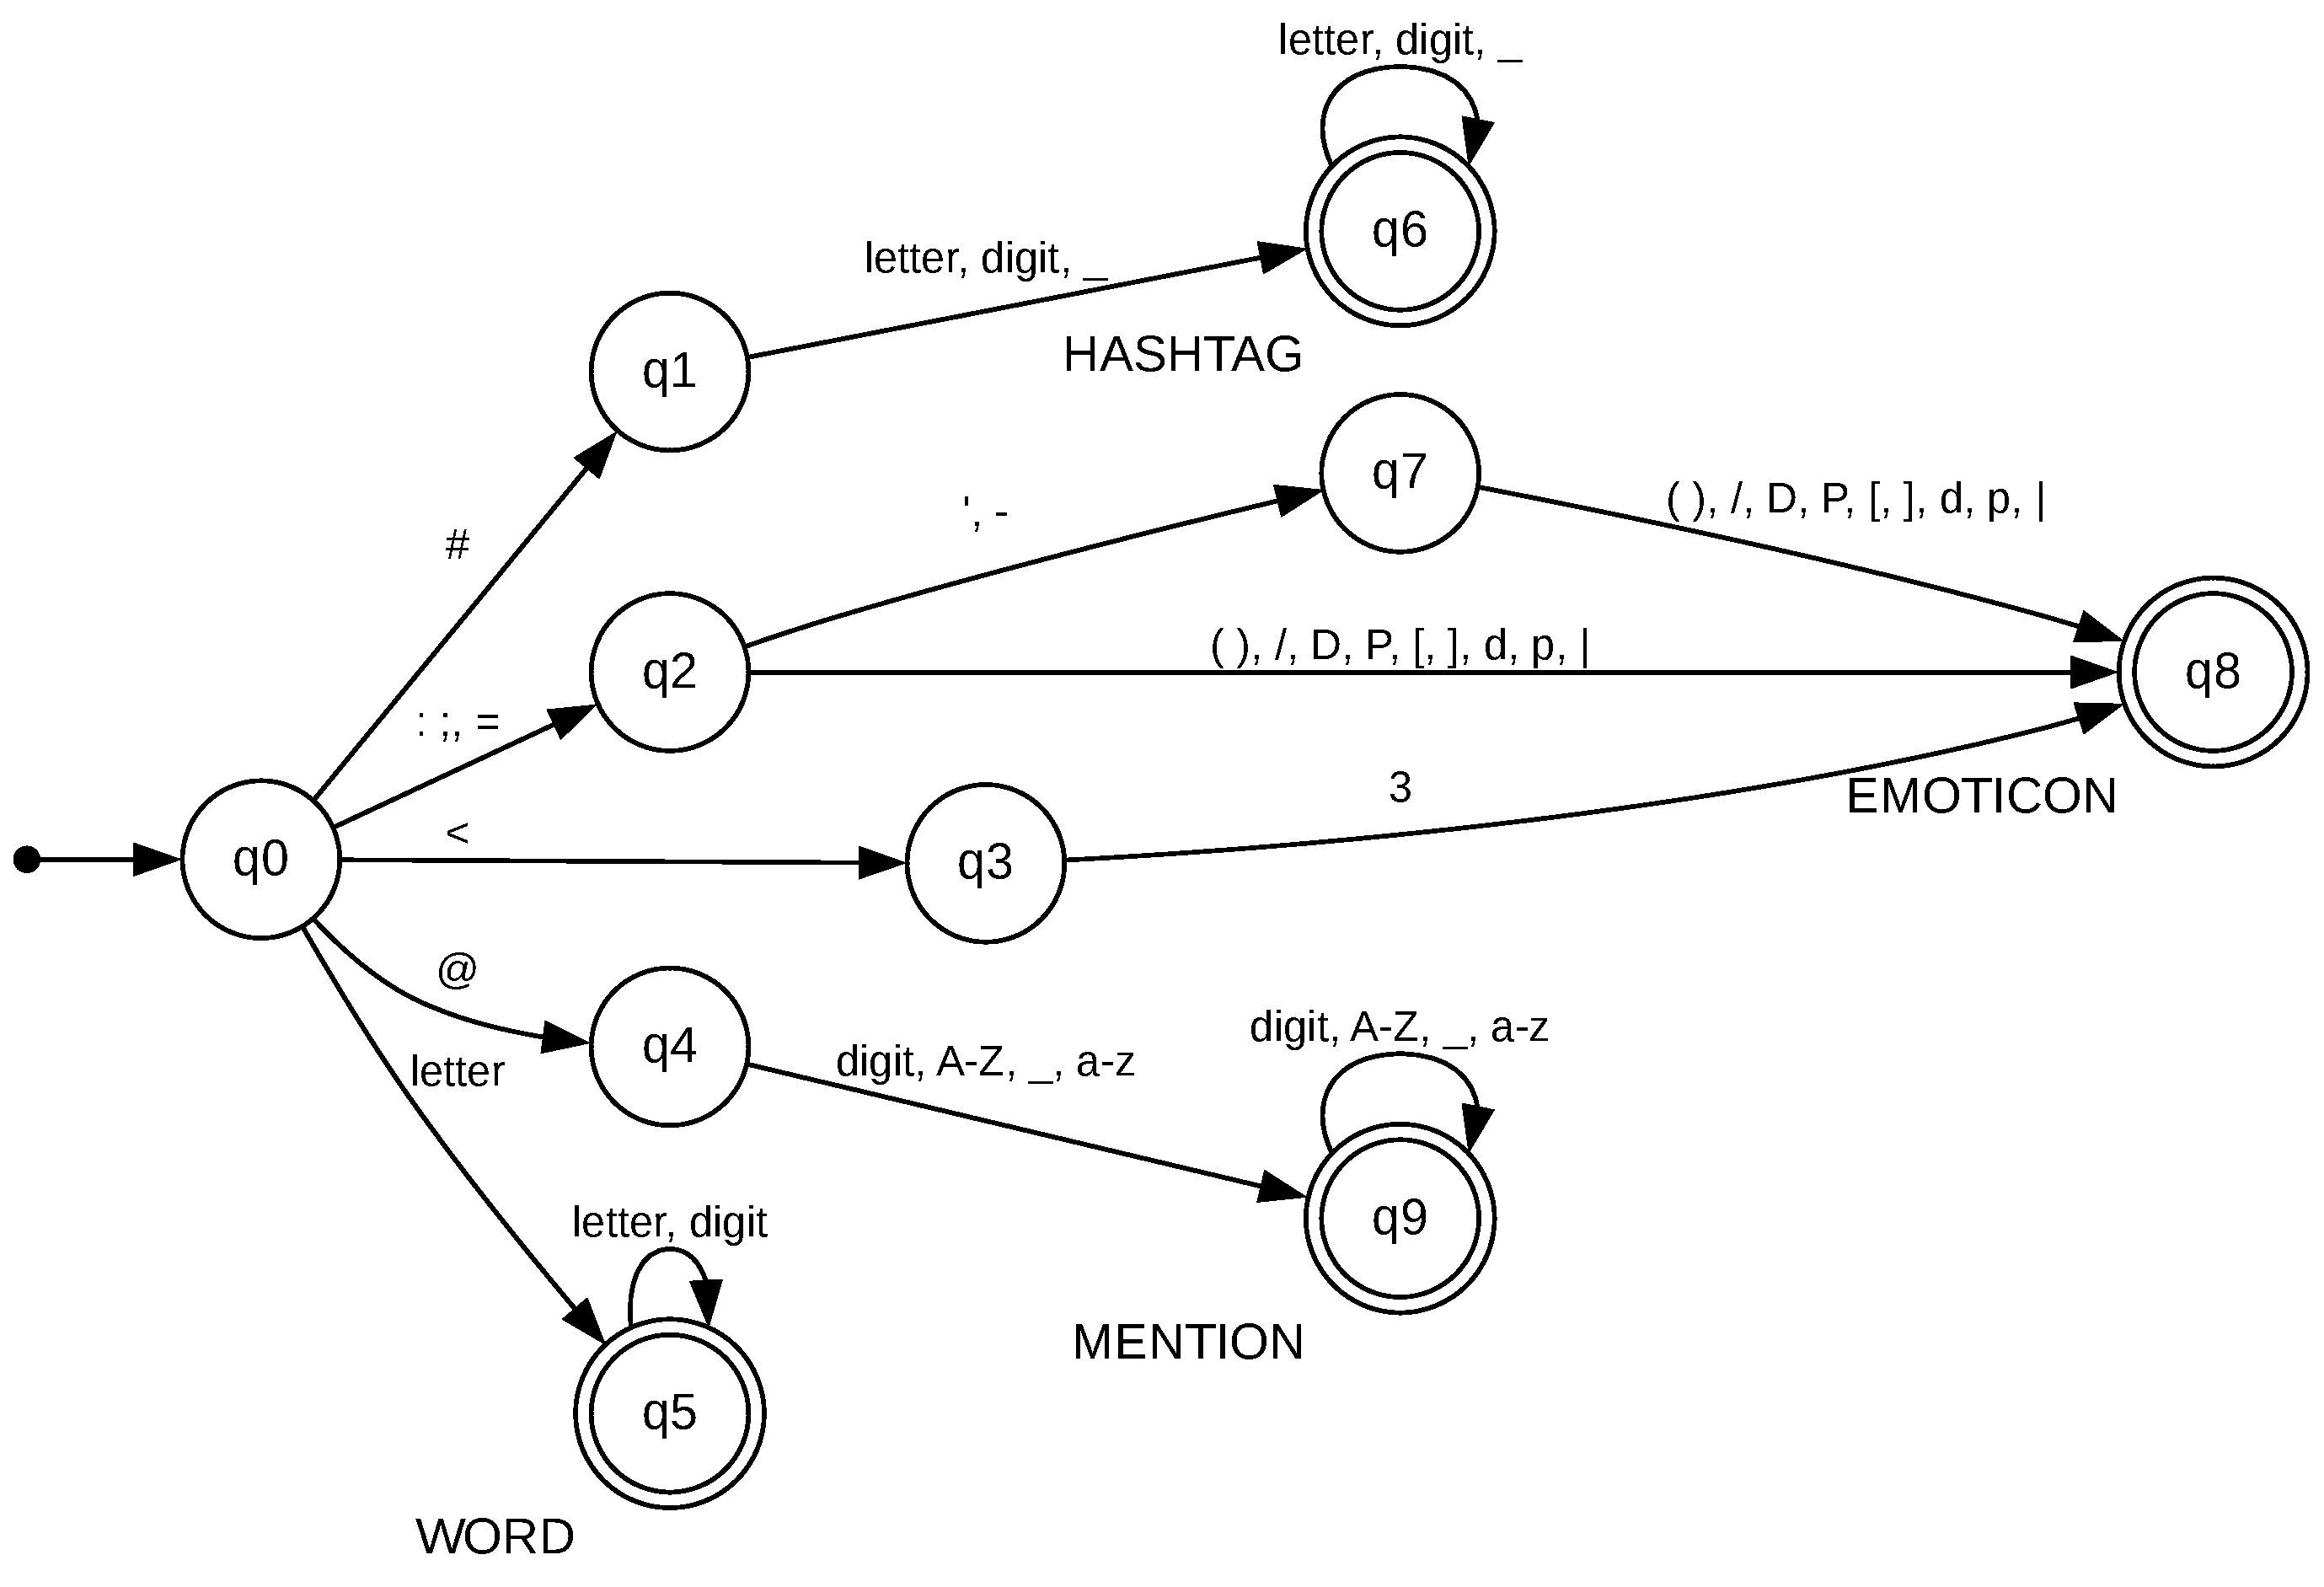
\includegraphics[width=0.6\columnwidth]{dfa_min}
\caption{The minimized combined DFA}\label{fig:3}
\end{figure}

\par\noindent\textit{Intrinsic metrics.}
Table~\ref{tab:4} compares the word-level tokenizers on three intrinsic measures. LexFront has the lowest out-of-vocabulary rate and the smallest vocabulary on all three datasets. On ag\_news, for example, its OOV rate is 0.48\% against 0.96\% for NLTK, and its vocabulary has 65,337 types against 98,994. We need to be careful with this result. Part of it is built in, because placeholders and collapsed letters shrink the vocabulary by design, so it is not evidence of better classification by itself. The accuracy results are the real check, and we look at them next.

\par\noindent\textit{Classification with LexFront.}
Table~\ref{tab:5} gives the main comparison. We call LexFront with Logistic Regression our proposed setup and NLTK with Naive Bayes the existing one. The proposed setup is 17.58 points higher on go\_emotions and 1.50 higher on ag\_news, and 0.26 lower on tweet\_topic, so on the surface it looks good. The last two columns separate the effects. NLTK with Logistic Regression scores about the same as LexFront with Logistic Regression on go\_emotions and ag\_news, which tells us that nearly all of the gain is the classifier and not the tokenizer. This is why we report the tokenizer-only comparison in Section~\ref{sec:5} as the fair one.

\subsection{Module 3: Normalizer and rule ablation}\label{sec:4.4}
Table~\ref{tab:6} shows the effect of removing one rule at a time in the main setting, where TF-IDF still lowercases the text. In this setting no single-rule removal gives an accuracy interval that excludes 0, so none of the individual rules shows a clear effect on its own. One more thing explains part of this. The URL rule never fires on tweet\_topic and go\_emotions, and the mention rule never fires on ag\_news, because those datasets already mask URLs and handles. For those cases the removal is not a real test of the rule. The one setting that does stand out is removing every rule on tweet\_topic, which raises accuracy by 1.09 points [+0.50, +1.71]. In other words, on that dataset the normalization as a whole does not help.

\begin{figure}[!t]
\centering
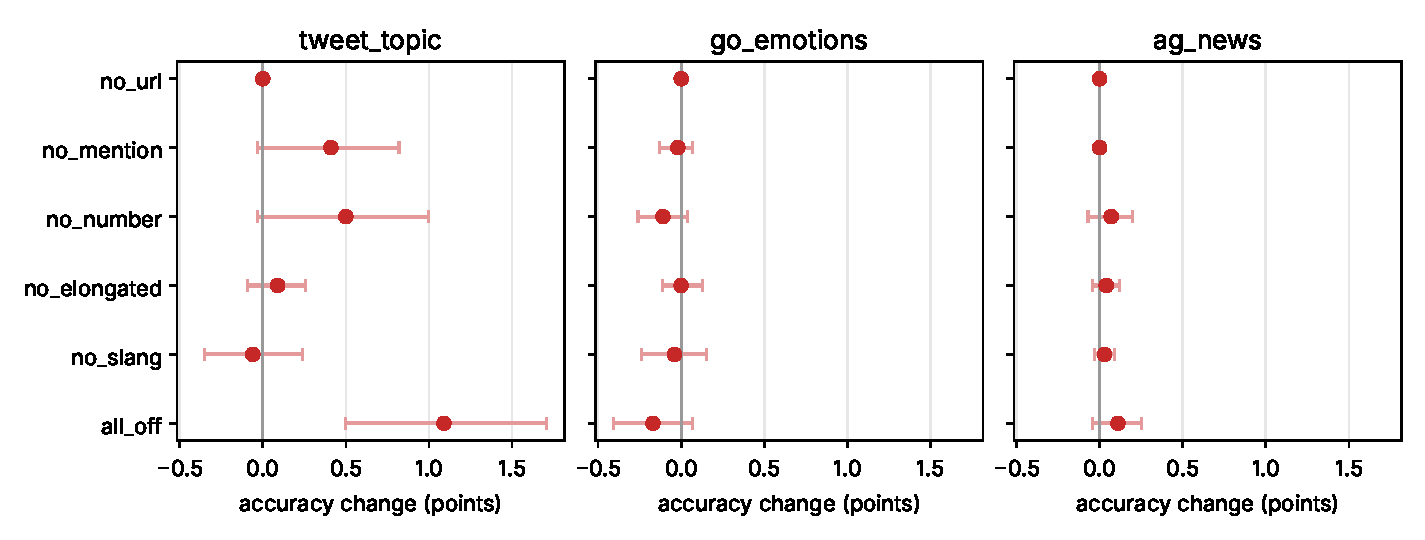
\includegraphics[width=\textwidth]{ablation}
\caption{Rule ablation: accuracy change with 95\% intervals (main setting)}\label{fig:4}
\end{figure}

The case-sensitivity check tells a clearer story. When TF-IDF's own lowercasing is switched off, the lowercase rule inside LexFront becomes the one that matters. Removing it lowers accuracy by 0.91 points on tweet\_topic [$-$1.71, $-$0.09] and by 1.07 on go\_emotions [$-$1.72, $-$0.44], while ag\_news does not change in a clear way (+0.14 [$-$0.17, +0.46]). The same check explains a result we noticed earlier. With case kept, LexFront barely moves, with Logistic Regression accuracy changing by only $-$0.03, $-$0.02 and +0.04 points on the three datasets, while the baseline tokenizers lose between 0.6 and 1.3 points on tweet\_topic and go\_emotions, because they leave capitalised words alone. With case kept, LexFront beats NLTK on go\_emotions by 1.15 points [+0.46, +1.85]. Our reading is that this advantage comes from the lowercase rule alone, and since TF-IDF lowercases by default, it disappears in the main setting.

\subsection{Module 4: Subword stage}\label{sec:4.5}
Table~\ref{tab:8} lists the subword runs next to the two word-level references. BPE with a vocabulary of 8,000 shows no accuracy gain over NLTK with Logistic Regression. The intervals include 0 on tweet\_topic ($-$0.41 [$-$1.27, +0.44]) and go\_emotions ($-$0.04 [$-$0.68, +0.59]), and on ag\_news it is 0.75 points lower [$-$1.13, $-$0.37]. The LexFront + BPE hybrid is below LexFront alone on all three datasets, by 0.82, 0.72 and 0.86 points, and 17 of the 24 intervals in the hybrid comparison at vocabulary 8,000 exclude 0, all pointing down. A bigger vocabulary (32,000) reduced this, since 8 of 24 intervals exclude 0 there. Our guess, which we have not tested, is that the hybrid splits up words that the word-level scanner already handled well, so it adds noise. For WordPiece and Unigram, none is above NLTK with Logistic Regression in accuracy with an interval that excludes 0, and on ag\_news both are below it ($-$0.41 and $-$0.91). The one interval that is above NLTK is Unigram's macro-F1 on go\_emotions (+1.26 [+0.10, +2.39]), which is 1 of 30 comparisons and could easily be chance.

\begin{figure}[!t]
\centering
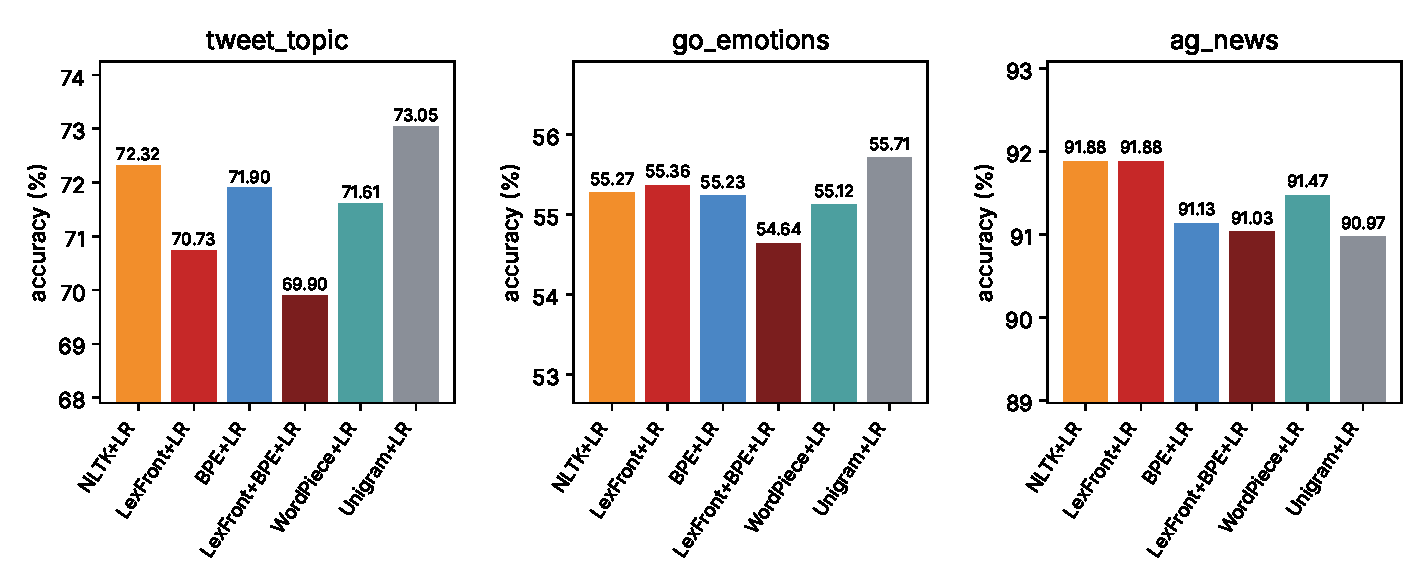
\includegraphics[width=\textwidth]{subword}
\caption{Accuracy of the subword tokenizers with Logistic Regression}\label{fig:5}
\end{figure}

The OOV rate of the subword tokenizers is close to zero, for example 0.44\% for BPE and 0.31\% for WordPiece on tweet\_topic, because rare words are split into pieces instead of being left unknown. That number is not comparable with the word-level OOV rates in Table~\ref{tab:4}, and the price is more tokens per word (fertility goes up to between 1.3 and 1.8).

\subsection{Module 5: Tuned classifiers on the eight-dataset collection}\label{sec:4.6}
The first question about the earlier results is whether they depend on the default classifier settings. To check, we cleaned eight datasets and tuned the classifier equally for every tokenizer, choosing the TF-IDF setting and C or alpha on a validation slice of the training data. Tuning raised accuracy in 44 of 64 dataset, tokenizer and classifier cells, lowered it in 16 and left 4 equal, with a mean change of +1.63 points. The largest gains are for Naive Bayes, for example +8.12 points on average over the tokenizers on go\_emotions and +10.26 on tweet\_eval emotion. Table~\ref{tab:9} shows what this does to the tokenizer comparison. With default settings, LexFront differs clearly from NLTK on 4 of the 8 datasets (two up and two down). With tuned settings, none of the 8 intervals excludes 0. In other words, tuning removes most of the differences that were visible at default settings, and the test sets of the small datasets are too small to show anything else. The one large positive value, tweet\_eval irony, rests on only 784 test examples and its interval just touches 0.

\subsection{Module 5: Large-scale test on Sentiment140}\label{sec:4.7}
Sentiment140 has 1.6 million tweets, which is enough to separate small differences from noise. We split by user (5\% of users held out, none in both splits), cleaned the data, and ran every tokenizer at default, validation-tuned and wide-tuned settings. The first part of Table~\ref{tab:10} is Logistic Regression and the second is Naive Bayes. At default settings the four tokenizers are close, with LexFront at 79.85 against 79.88 for NLTK. With tuned settings every tokenizer gains about 2 to 3 points, and LexFront is highest by a small amount (82.84 against 82.73 for NLTK with the wide setting). The paired differences are small. For Logistic Regression, LexFront minus NLTK is $-$0.03 [$-$0.16, +0.10] at default settings, +0.17 [0.00, +0.34] tuned and +0.11 [$-$0.04, +0.25] wide, all inside the 0.5-point margin. The size ladder shows the same: the mean LexFront minus NLTK gap is +0.12 at 10,000 training examples, +0.10 at 100,000, +0.09 at one million and $-$0.03 on the full set, so it shrinks toward zero as data grows.

\begin{table}[!tb]
\caption{Sentiment140 test accuracy (\%), word tokenizers and the character n-gram baseline}\label{tab:10}
\centering
\footnotesize
\setlength{\tabcolsep}{4pt}
\begin{tabular}{lllllll}
\toprule
\textbf{Tokenizer} & \textbf{LR default} & \textbf{LR tuned} & \textbf{LR wide} & \textbf{NB default} & \textbf{NB tuned} & \textbf{NB wide} \\
\midrule
whitespace & 79.60 & 81.44 & 81.68 & 76.80 & 80.19 & 80.53 \\
nltk & 79.88 & 82.37 & 82.73 & 77.05 & 80.34 & 80.31 \\
tweet & 79.96 & 82.23 & 82.50 & 77.11 & 80.52 & 80.52 \\
lexfront & 79.85 & 82.54 & 82.84 & 77.33 & 80.49 & 80.49 \\
char n-grams & - & - & 80.11 & - & - & 75.22 \\
\bottomrule
\end{tabular}
\end{table}

Two other results from this run are worth reporting. First, in the noise test the tokenizers lose accuracy as expected, and LexFront loses the least (Table~\ref{tab:11}). With heavy noise, LexFront minus NLTK is +0.14 points, and the difference in accuracy lost is +0.16 [+0.02, +0.32], which is a small effect, well inside the margin, but its interval excludes 0. Second, the character n-gram baseline, which we expected to be a strong competitor for noisy text, is clearly worse here: with wide settings it is 2.74 points below LexFront for Logistic Regression and 5.26 points below for Naive Bayes.

On the practical side, at default settings LexFront produced 104,503 features against 228,086 for NLTK and 226,995 for TweetTokenizer, and tokenized 6,566 test tweets per second, against 4,845 for NLTK, 10,542 for TweetTokenizer and about 1.08 million for whitespace splitting. So it is faster than NLTK and slower than TweetTokenizer on this machine.

\subsection{Module 5: Wider settings and the character baseline}\label{sec:4.8}
The wide setting in Table~\ref{tab:10} is a larger validated grid (word n-grams up to 3, plain or sublinear term frequency, minimum document frequency 2 or 5, and wider C and alpha ranges) that we applied equally to every tokenizer. Compared with default settings, it adds +2.01 points for whitespace, +2.86 for NLTK, +2.57 for TweetTokenizer and +3.00 for LexFront with Logistic Regression, and +3.2 to +3.7 points with Naive Bayes. Compared with the earlier tuned setting the extra gain is small (+0.24 to +0.37 for Logistic Regression). The gain from tuning therefore dwarfs any difference between the word tokenizers. Of the five hypotheses we wrote down for this phase, only one was observed: LexFront stayed within the margin of NLTK and TweetTokenizer. The others were not (Section~\ref{sec:5.6}).

\subsection{Module 5: Civil Comments, Amazon polarity and Yelp}\label{sec:4.9}
To see whether Sentiment140 is typical, we ran the same protocol on three more large datasets: Civil Comments and Amazon polarity with about 500,000 training examples each, and Yelp with about 300,000. Civil Comments is a comments dataset where the toxic class is rare (the majority class alone gives 92.02\% accuracy), so we use macro-F1 as the primary metric there. Amazon polarity is clean review text and acts as a control. Table~\ref{tab:12} gives the wide-tuned results. On Civil Comments, LexFront, NLTK and TweetTokenizer are essentially tied, and all three are clearly ahead of whitespace splitting in macro-F1: LexFront minus whitespace is +2.25 points [+1.79, +2.70] for Logistic Regression, and with default settings +4.03. On Amazon, LexFront and TweetTokenizer are level with each other ($-$0.01 [$-$0.09, +0.07]) and both are ahead of NLTK, with LexFront minus NLTK at +0.46 [+0.34, +0.57]. That interval is above zero but crosses the 0.5-point margin, so we label it unclear and not a clear gain. Wider settings help a lot here: +2.8 to +3.3 points for Logistic Regression and +5.7 to +6.7 for Naive Bayes on Amazon.

Yelp has five star classes (balanced, so the majority class gives 20.00\%), which makes it the one many-class large test. The result is again the same. With wide settings and Logistic Regression, LexFront minus NLTK is +0.07 points [$-$0.16, +0.31] and LexFront minus TweetTokenizer is $-$0.15 [$-$0.37, +0.07], both inside the margin, while LexFront is +1.08 [+0.76, +1.38] ahead of whitespace splitting, which is beyond the margin. With Naive Bayes, LexFront minus NLTK is $-$0.09 [$-$0.28, +0.11]. Wide settings add +2.63 to +3.15 points for Logistic Regression and +5.4 to +6.3 for Naive Bayes compared with default settings, again much more than any difference between the word tokenizers.

\begin{table}[!tb]
\caption{Wide-tuned test results, accuracy / macro-F1 (\%)}\label{tab:12}
\centering
\footnotesize
\setlength{\tabcolsep}{4pt}
\begin{tabular}{llllll}
\toprule
\textbf{Dataset} & \textbf{Tokenizer} & \textbf{LR accuracy} & \textbf{LR macro-F1} & \textbf{NB accuracy} & \textbf{NB macro-F1} \\
\midrule
Civil Comments & whitespace & 94.39 & 76.85 & 92.95 & 61.08 \\
Civil Comments & nltk & 94.67 & 79.04 & 93.24 & 64.49 \\
Civil Comments & tweet & 94.63 & 78.98 & 93.24 & 64.60 \\
Civil Comments & lexfront & 94.66 & 79.09 & 93.30 & 65.04 \\
Amazon polarity & whitespace & 93.28 & 93.28 & 91.01 & 91.01 \\
Amazon polarity & nltk & 93.32 & 93.32 & 91.24 & 91.24 \\
Amazon polarity & tweet & 93.78 & 93.78 & 91.35 & 91.35 \\
Amazon polarity & lexfront & 93.77 & 93.77 & 91.31 & 91.31 \\
Yelp & whitespace & 61.67 & 61.51 & 58.54 & 58.60 \\
Yelp & nltk & 62.67 & 62.53 & 59.20 & 59.29 \\
Yelp & tweet & 62.89 & 62.76 & 59.42 & 59.51 \\
Yelp & lexfront & 62.75 & 62.60 & 59.11 & 59.21 \\
\bottomrule
\end{tabular}
\end{table}

A caution on how these three runs were made. They ran on a Windows laptop with Python 3.12, while the Sentiment140 runs ran on Colab. Each run records its own library versions, so the results are valid but should not be mixed at the digit level. The Yelp run needed about 10 hours of fitting time in total, and an earlier attempt on Colab did not finish.

\section{Performance and Metrics}\label{sec:5}
This section pulls the comparison together. We use two metrics, accuracy and macro-F1. Macro-F1 matters on tweet\_topic and go\_emotions, where the classes are unbalanced, because a model can have decent accuracy by favouring the large classes. We also report paired 95\% bootstrap intervals and McNemar's test, so that each difference comes with a statement of how large the test-set noise is.

\subsection{Accuracy: existing versus proposed}\label{sec:5.1}
\begin{figure}[!t]
\centering
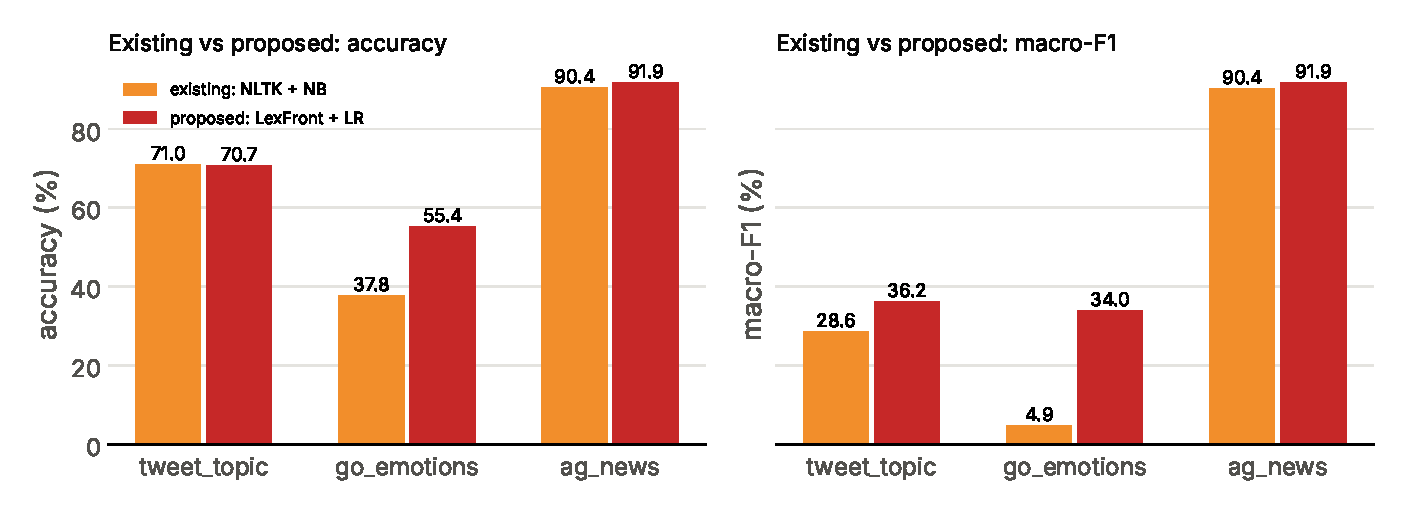
\includegraphics[width=\textwidth]{hq_existing_vs_proposed}
\caption{Existing (NLTK+NB) versus proposed (LexFront+LR), accuracy and macro-F1}\label{fig:6}
\end{figure}

Fig.~\ref{fig:6} shows the headline comparison, which is the same one as in Table~\ref{tab:5}. The proposed setup is higher on go\_emotions and ag\_news and about level on tweet\_topic in accuracy. In macro-F1 it is higher on all three, by 7.62 points on tweet\_topic and 29.09 on go\_emotions. The tokenizer-only comparison in Table~\ref{tab:13} shows where that comes from.

\subsection{Separating the tokenizer from the classifier}\label{sec:5.2}
\begin{table}[!tb]
\caption{Paired differences, accuracy points [95\% CI]}\label{tab:13}
\centering
\footnotesize
\setlength{\tabcolsep}{4pt}
\begin{tabularx}{\textwidth}{lYlll}
\toprule
\textbf{Dataset} & \textbf{Comparison} & \textbf{Accuracy pts [95\% CI]} & \textbf{Macro-F1 pts [95\% CI]} & \textbf{McNemar p} \\
\midrule
tweet\_topic & LexFront+LR minus NLTK+LR (tokenizer only) & $-$1.59 [$-$2.38, $-$0.82] & $-$0.77 [$-$1.81, +0.32] & \textless{} 0.001 \\
tweet\_topic & LexFront+LR minus NLTK+NB (proposed minus existing) & $-$0.26 [$-$1.47, +0.91] & +7.62 [+5.93, +9.31] & - \\
go\_emotions & LexFront+LR minus NLTK+LR (tokenizer only) & +0.09 [$-$0.35, +0.54] & +0.11 [$-$0.51, +0.77] & 0.773 \\
go\_emotions & LexFront+LR minus NLTK+NB (proposed minus existing) & +17.58 [+16.21, +18.95] & +29.09 [+27.32, +31.07] & - \\
ag\_news & LexFront+LR minus NLTK+LR (tokenizer only) & +0.00 [$-$0.32, +0.33] & $-$0.01 [$-$0.33, +0.33] & 1.000 \\
ag\_news & LexFront+LR minus NLTK+NB (proposed minus existing) & +1.50 [+1.00, +1.99] & +1.51 [+1.01, +2.01] & - \\
\bottomrule
\end{tabularx}
\end{table}

Reading Table~\ref{tab:13} row by row, the tokenizer-only differences are the fair test of LexFront. On go\_emotions and ag\_news the intervals include 0, so LexFront and NLTK are indistinguishable there. On tweet\_topic LexFront is 1.59 points lower and that difference is significant (McNemar p \textless{} 0.001). The proposed-minus-existing rows are large on go\_emotions and ag\_news, but almost all of that is the move from Naive Bayes to Logistic Regression: with NLTK held fixed, the classifier change alone is worth +17.49 on go\_emotions and +1.50 on ag\_news. So we do not claim that LexFront is better. What the data support is that it does about as well as NLTK on two of the datasets and somewhat worse on one, and that it gives a smaller vocabulary and a lower OOV rate.

\subsection{Across all datasets}\label{sec:5.3}
\begin{figure}[!t]
\centering
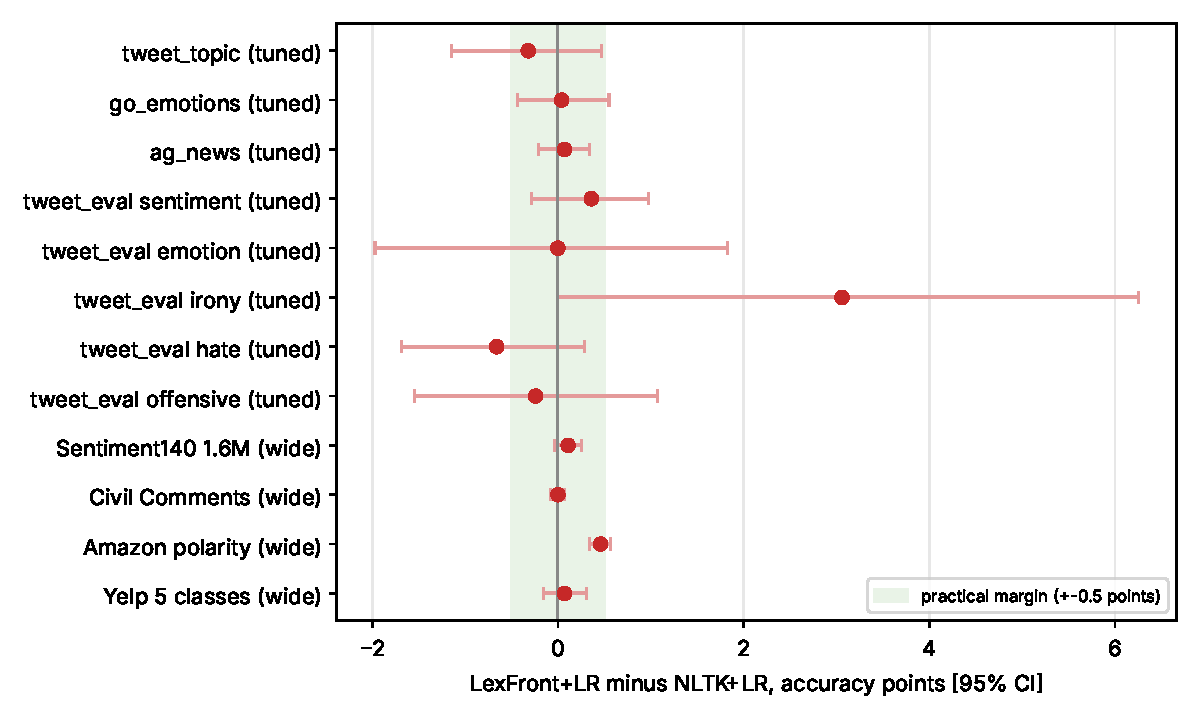
\includegraphics[width=0.78\columnwidth]{forest}
\caption{LexFront+LR minus NLTK+LR, accuracy points with 95\% intervals; the green band is the plus or minus 0.5 point practical margin}\label{fig:7}
\end{figure}

Fig.~\ref{fig:7} puts the tokenizer-only comparison for Logistic Regression on all twelve datasets in one place. The tuned or wide-tuned setting is used, so that the comparison is not tied to default settings. The picture is clear. Ten of the twelve point estimates lie inside the margin. The two exceptions are tweet\_eval hate ($-$0.66) and irony (+3.06), and both have wide intervals that include values inside the margin. The four large datasets have much narrower intervals, and they are tight around zero: +0.11 on Sentiment140, 0.00 on Civil Comments, +0.46 on Amazon polarity and +0.07 on Yelp. The small datasets have wide intervals, because their test sets are small, so they cannot rule out a difference of a point or more in either direction. The only point far from zero, tweet\_eval irony, has the widest interval and rests on 784 test examples. There is no dataset where LexFront is clearly better than NLTK by more than the margin, and none where it is clearly worse once the classifier is tuned. We read this as ``competitive'', not ``better''.

\subsection{Intrinsic measures and speed}\label{sec:5.4}
On the intrinsic side, LexFront has the lowest OOV rate and the smallest vocabulary among the word-level tokenizers on the three core datasets, with fertility close to the others. On Sentiment140 it also gives the smallest feature set. Part of this is built in, because placeholders and collapsed letters shrink the vocabulary by design, so it is a description and not evidence of better classification. Speed is in the same range as the other tokenizers. On the core datasets it runs at about 0.84 to 1.48 times the speed of NLTK, and on Sentiment140 at 6,566 tweets per second against 4,845 for NLTK. The lexer is therefore not a bottleneck. The subword tokenizers (Fig.~\ref{fig:5} and Table~\ref{tab:8}) are not clearly better than NLTK in accuracy on the core datasets, and the character n-gram baseline is clearly worse on Sentiment140.

\subsection{Where the accuracy comes from}\label{sec:5.5}
Table~\ref{tab:14} compares the size of the different changes we tried. The pattern is consistent across datasets. The classifier and its tuning move accuracy by several points, and the tokenizer moves it by a fraction of a point once the classifier is tuned. This is the main finding of the project, and it is more useful than a single headline number.

\begin{table}[!tb]
\caption{Size of each change in accuracy points (from the tables above)}\label{tab:14}
\centering
\footnotesize
\setlength{\tabcolsep}{3pt}
\begin{tabularx}{\textwidth}{YYl}
\toprule
\textbf{Change} & \textbf{Typical effect} & \textbf{Where} \\
\midrule
Naive Bayes to Logistic Regression (NLTK, default settings) & +1.32 to +17.49 & Table~\ref{tab:13}, core datasets \\
Default to tuned settings, Naive Bayes & $-$1.01 to +10.26 (mean over tokenizers, collection); +5.4 to +6.7 on Amazon and Yelp & Sections~\ref{sec:4.6}, \ref{sec:4.9} \\
Default to tuned settings, Logistic Regression & $-$0.77 to +1.41 (collection); +2.0 to +3.0 (Sentiment140); +2.8 to +3.3 (Amazon); +2.6 to +3.2 (Yelp) & Sections~\ref{sec:4.6} to \ref{sec:4.9} \\
LexFront versus NLTK, Logistic Regression, tuned & 0.00 to +0.46 on the four large datasets; $-$0.66 to +3.06 (wide intervals) on the small ones & Fig.~\ref{fig:7} \\
LexFront versus whitespace, Logistic Regression & +0.27 to +1.17 accuracy; +2.25 macro-F1 on Civil Comments & Sections~\ref{sec:4.7} to \ref{sec:4.9} \\
Character n-grams versus LexFront (Sentiment140) & $-$2.74 (Logistic Regression), $-$5.26 (Naive Bayes) & Section~\ref{sec:4.7} \\
\bottomrule
\end{tabularx}
\end{table}

\subsection{Hypotheses written before the runs}\label{sec:5.6}
Because we wrote hypotheses and a decision rule before each large run, we can say which ones held. Table~\ref{tab:15} lists them. Several of our own expectations were not supported, and we report them as such. For example, we expected wider tuning to push every tokenizer beyond the earlier tuned setting (HA1), and it did not, and we expected the character n-gram baseline to be at least as good as LexFront (HA4), and it was clearly worse.

\begin{table}[!tb]
\caption{Outcome of the pre-registered hypotheses}\label{tab:15}
\centering
\footnotesize
\setlength{\tabcolsep}{3pt}
\begin{tabularx}{\textwidth}{lYY}
\toprule
\textbf{Hypothesis} & \textbf{Statement (short)} & \textbf{Outcome} \\
\midrule
H1 (Sentiment140) & LexFront minus NLTK gap is smaller at full data than at 10,000 examples & Observed (+0.12 against $-$0.03) \\
H2 (Sentiment140) & LexFront loses less accuracy than NLTK under heavy noise & Observed (+0.16 [+0.02, +0.32]) \\
H3 (Sentiment140) & The gap is smaller with tuned than with default settings & Not observed ($-$0.03 against +0.17) \\
HA1 (Sentiment140) & Wide tuning beats the earlier tuned setting beyond the margin for every tokenizer & Not observed \\
HA2 (Sentiment140) & With wide tuning LexFront is within the margin of NLTK and TweetTokenizer & Observed \\
HA3 (Sentiment140) & The spread across tokenizers is smaller when wide-tuned & Not observed (1.17 against 0.26) \\
HA4 (Sentiment140) & Character n-grams are within or above LexFront & Opposite: 2.74 points below \\
HA5 (Sentiment140) & Wide NB LexFront is beyond the earlier tuned NB & Not observed \\
HA2 / HA3 (Civil Comments) & As above & Both observed \\
HA2 / HA3 (Amazon polarity) & As above & Neither observed (LexFront minus NLTK +0.46 is unclear) \\
HA2 / HA3 (Yelp) & As above & HA2 observed, HA3 not observed (1.22 against 0.98) \\
\bottomrule
\end{tabularx}
\end{table}

\subsection{Limits of these measurements}\label{sec:5.7}
A few cautions apply to all of the numbers. There is one training run per cell, so training randomness is not covered by the intervals, which only measure test-set sampling. We ran many comparisons and did not correct for multiple testing. In the rule ablation, 6 of 42 interval comparisons exclude 0 when about 2 would be expected by chance. All datasets are English, and all large ones except Yelp are two-class, so we cannot say anything about other languages or code-mixed text, and Yelp is our only many-class test at scale. We did not test transformer models. The Colab and laptop runs used different library versions, which each run records. All reasons we give for why a difference appears are hypotheses, not tested conclusions.

\section{Conclusion}\label{sec:6}
We built LexFront, a compiler-style lexer for noisy English text, with our own regex-to-DFA engine, a normalizer with six switchable rules, a symbol table and error recovery, and compared it with existing and subword tokenizers under a fixed classifier. The engine works as intended: the combined automaton goes from 43 NFA states to 12 DFA states and 10 minimized states, and it agrees with the PLY lexer on the four classes it covers. The classification experiments themselves run on the PLY-based lexer.

On the question we started with, the answer is that a compiler-style lexer is competitive but not better. This held on the three core datasets, on the eight-dataset collection with fair tuning, and on four large datasets with about 300,000 to 1.5 million training examples, one of them with five classes. With the tokenizer as the only change, LexFront stays within about half a point of NLTK and TweetTokenizer on the large datasets, and its clear advantage is over plain whitespace splitting, especially in macro-F1 on Civil Comments and by about one point on Yelp. It gives a smaller vocabulary, a lower out-of-vocabulary rate and slightly smaller accuracy losses under added noise. Most of the accuracy comes from the classifier and its tuning. BPE, WordPiece, Unigram and the character n-gram baseline did not improve on the word-level tokenizers, and several of our own hypotheses were not supported, which we report as they came out.

The main limits are one training run per cell, English-only data, and no transformer baseline. Natural next steps are repeating the large runs with other random seeds, running the character baseline on the two newer datasets, testing across domains (training on one source and testing on another), and trying a tweet-trained transformer model, which would use its own tokenizer and therefore test a different question.

\begin{table}[!t]
\centering
{\footnotesize APPENDIX A}\\[1pt]{\footnotesize\textsc{Additional results}}\par\vspace{6pt}
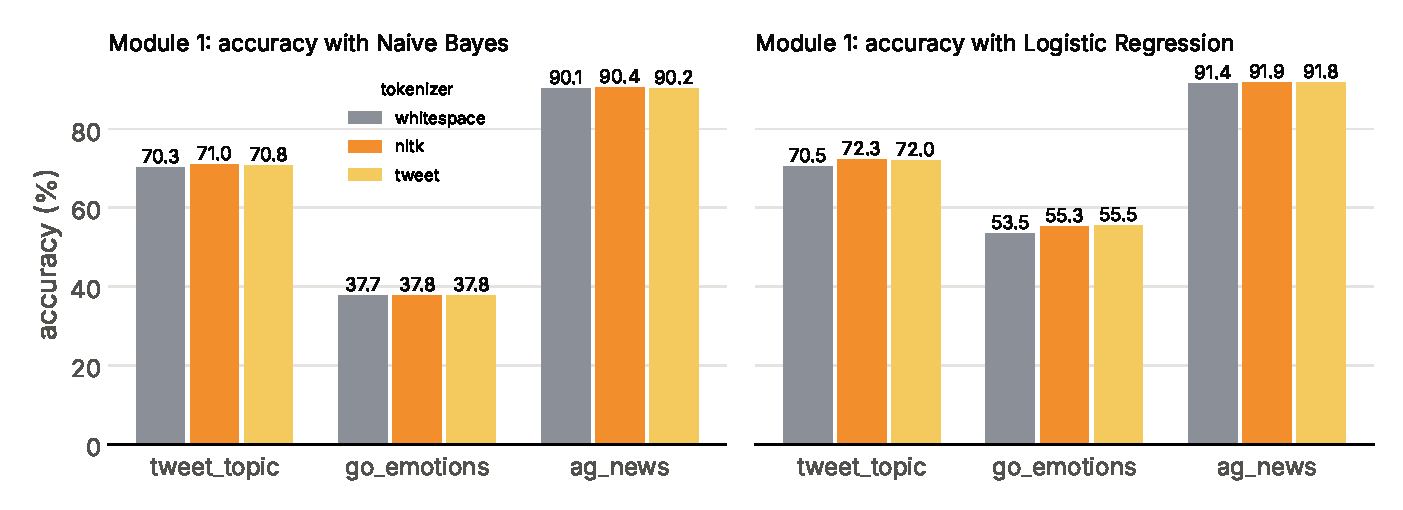
\includegraphics[width=0.74\textwidth]{hq_module1_accuracy}\par\refstepcounter{figure}\label{fig:2}{\footnotesize Fig.~\thefigure.\ Accuracy of the existing tokenizers}\par\vspace{6pt}
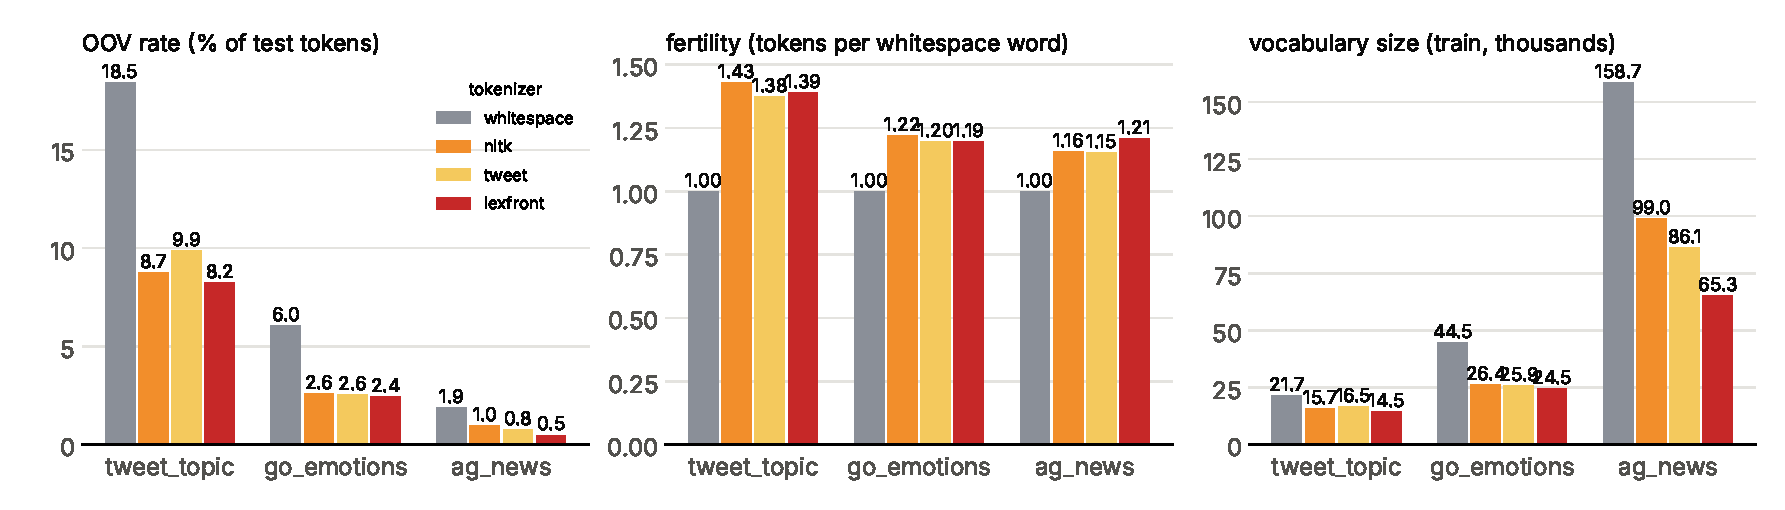
\includegraphics[width=0.74\textwidth]{hq_intrinsic_metrics}\par\refstepcounter{figure}\label{fig:8}{\footnotesize Fig.~\thefigure.\ OOV rate, fertility and vocabulary size by tokenizer}\par\vspace{6pt}
\end{table}

\begin{table}[!t]
\centering
\begin{minipage}[t]{0.485\textwidth}
\refstepcounter{table}\label{tab:2}\begin{center}{\footnotesize TABLE~\thetable}\\[1pt]{\footnotesize\textsc{Accuracy / macro-F1 (\%), existing tokenizers}}\\[3pt]
\footnotesize
\setlength{\tabcolsep}{4pt}
\adjustbox{max width=\columnwidth}{%
\begin{tabular}{lllll}
\toprule
\textbf{Dataset} & \textbf{Tokenizer} & \textbf{Majority} & \textbf{Naive Bayes} & \textbf{Logistic Reg.} \\
\midrule
tweet\_topic & whitespace & 40.01 / 9.53 & 70.26 / 28.83 & 70.49 / 35.76 \\
tweet\_topic & nltk & 40.01 / 9.53 & 70.99 / 28.56 & 72.32 / 36.95 \\
tweet\_topic & tweet & 40.01 / 9.53 & 70.79 / 28.31 & 72.02 / 36.70 \\
go\_emotions & whitespace & 34.99 / 1.85 & 37.73 / 4.93 & 53.51 / 31.40 \\
go\_emotions & nltk & 34.99 / 1.85 & 37.78 / 4.88 & 55.27 / 33.86 \\
go\_emotions & tweet & 34.99 / 1.85 & 37.80 / 4.86 & 55.47 / 34.02 \\
ag\_news & whitespace & 25.00 / 10.00 & 90.14 / 90.12 & 91.43 / 91.42 \\
ag\_news & nltk & 25.00 / 10.00 & 90.38 / 90.35 & 91.88 / 91.87 \\
ag\_news & tweet & 25.00 / 10.00 & 90.22 / 90.20 & 91.84 / 91.83 \\
\bottomrule
\end{tabular}
}
\end{center}\vspace{4pt}
\refstepcounter{table}\label{tab:4}\begin{center}{\footnotesize TABLE~\thetable}\\[1pt]{\footnotesize\textsc{Intrinsic metrics of the word-level tokenizers}}\\[3pt]
\footnotesize
\setlength{\tabcolsep}{4pt}
\adjustbox{max width=\columnwidth}{%
\begin{tabular}{lllll}
\toprule
\textbf{Dataset} & \textbf{Tokenizer} & \textbf{OOV rate \% (tokens)} & \textbf{Fertility} & \textbf{Vocabulary size} \\
\midrule
tweet\_topic & whitespace & 18.45 & 1.000 & 21,653 \\
tweet\_topic & nltk & 8.74 & 1.431 & 15,712 \\
tweet\_topic & tweet & 9.86 & 1.376 & 16,524 \\
tweet\_topic & lexfront & 8.25 & 1.391 & 14,483 \\
go\_emotions & whitespace & 6.04 & 1.000 & 44,476 \\
go\_emotions & nltk & 2.57 & 1.220 & 26,410 \\
go\_emotions & tweet & 2.56 & 1.195 & 25,907 \\
go\_emotions & lexfront & 2.45 & 1.195 & 24,459 \\
ag\_news & whitespace & 1.90 & 1.000 & 158,733 \\
ag\_news & nltk & 0.96 & 1.158 & 98,994 \\
ag\_news & tweet & 0.75 & 1.154 & 86,096 \\
ag\_news & lexfront & 0.48 & 1.207 & 65,337 \\
\bottomrule
\end{tabular}
}
\end{center}\vspace{4pt}
\refstepcounter{table}\label{tab:5}\begin{center}{\footnotesize TABLE~\thetable}\\[1pt]{\footnotesize\textsc{Proposed (LexFront+LR) versus existing (NLTK+NB), accuracy / macro-F1 (\%)}}\\[3pt]
\footnotesize
\setlength{\tabcolsep}{4pt}
\adjustbox{max width=\columnwidth}{%
\begin{tabular}{llllll}
\toprule
\textbf{Dataset} & \textbf{NLTK+NB} & \textbf{LexFront+LR} & \textbf{Delta acc (pts)} & \textbf{LexFront+NB} & \textbf{NLTK+LR} \\
\midrule
tweet\_topic & 70.99 / 28.56 & 70.73 / 36.18 & $-$0.26 & 70.43 / 27.84 & 72.32 / 36.95 \\
go\_emotions & 37.78 / 4.88 & 55.36 / 33.97 & +17.58 & 37.78 / 4.81 & 55.27 / 33.86 \\
ag\_news & 90.38 / 90.35 & 91.88 / 91.86 & +1.50 & 90.08 / 90.05 & 91.88 / 91.87 \\
\bottomrule
\end{tabular}
}
\end{center}\vspace{4pt}
\refstepcounter{table}\label{tab:6}\begin{center}{\footnotesize TABLE~\thetable}\\[1pt]{\footnotesize\textsc{Per-rule ablation, accuracy change versus full LexFront+LR (points, 95\% CI), main setting}}\\[3pt]
\footnotesize
\setlength{\tabcolsep}{4pt}
\adjustbox{max width=\columnwidth}{%
\begin{tabular}{llll}
\toprule
\textbf{Variant removed} & \textbf{tweet\_topic} & \textbf{go\_emotions} & \textbf{ag\_news} \\
\midrule
url & +0.00 [+0.00, +0.00] & +0.00 [+0.00, +0.00] & +0.01 [$-$0.07, +0.09] \\
mention & +0.41 [$-$0.03, +0.82] & $-$0.02 [$-$0.13, +0.07] & +0.00 [+0.00, +0.00] \\
number & +0.50 [$-$0.03, +1.00] & $-$0.11 [$-$0.26, +0.04] & +0.07 [$-$0.07, +0.20] \\
elongated & +0.09 [$-$0.09, +0.26] & +0.00 [$-$0.11, +0.13] & +0.04 [$-$0.04, +0.12] \\
slang & $-$0.06 [$-$0.35, +0.24] & $-$0.04 [$-$0.24, +0.15] & +0.03 [$-$0.03, +0.09] \\
all rules off & +1.09 [+0.50, +1.71] & $-$0.17 [$-$0.41, +0.07] & +0.11 [$-$0.04, +0.25] \\
\bottomrule
\end{tabular}
}
\end{center}\vspace{4pt}
\end{minipage}\hfill\begin{minipage}[t]{0.485\textwidth}
\refstepcounter{table}\label{tab:7}\begin{center}{\footnotesize TABLE~\thetable}\\[1pt]{\footnotesize\textsc{Case kept (TF-IDF lowercase=False): LexFront+LR minus NLTK+LR, accuracy points [95\% CI]}}\\[3pt]
\footnotesize
\setlength{\tabcolsep}{3pt}
\adjustbox{max width=\columnwidth}{%
\begin{tabular}{lll}
\toprule
\textbf{Dataset} & \textbf{Case kept} & \textbf{Main setting} \\
\midrule
tweet\_topic & $-$0.91 [$-$1.88, +0.09] & $-$1.59 [$-$2.38, $-$0.82] \\
go\_emotions & +1.15 [+0.46, +1.85] & +0.09 [$-$0.35, +0.54] \\
ag\_news & $-$0.18 [$-$0.55, +0.20] & +0.00 [$-$0.32, +0.33] \\
\bottomrule
\end{tabular}
}
\end{center}\vspace{4pt}
\refstepcounter{table}\label{tab:8}\begin{center}{\footnotesize TABLE~\thetable}\\[1pt]{\footnotesize\textsc{Subword runs, Logistic Regression, accuracy / macro-F1 (\%), vocabulary 8000}}\\[3pt]
\footnotesize
\setlength{\tabcolsep}{4pt}
\adjustbox{max width=\columnwidth}{%
\begin{tabular}{lllllll}
\toprule
\textbf{Dataset} & \textbf{NLTK+LR} & \textbf{LexFront+LR} & \textbf{BPE+LR} & \textbf{LexFront+BPE+LR} & \textbf{WordPiece+LR} & \textbf{Unigram+LR} \\
\midrule
tweet\_topic & 72.32 / 36.95 & 70.73 / 36.18 & 71.90 / 35.09 & 69.90 / 33.56 & 71.61 / 34.88 & 73.05 / 36.49 \\
go\_emotions & 55.27 / 33.86 & 55.36 / 33.97 & 55.23 / 33.29 & 54.64 / 32.59 & 55.12 / 33.12 & 55.71 / 35.12 \\
ag\_news & 91.88 / 91.87 & 91.88 / 91.86 & 91.13 / 91.12 & 91.03 / 91.01 & 91.47 / 91.46 & 90.97 / 90.96 \\
\bottomrule
\end{tabular}
}
\end{center}\vspace{4pt}
\refstepcounter{table}\label{tab:9}\begin{center}{\footnotesize TABLE~\thetable}\\[1pt]{\footnotesize\textsc{LexFront+LR minus NLTK+LR, accuracy points [95\% CI]; * = interval excludes 0}}\\[3pt]
\footnotesize
\setlength{\tabcolsep}{3pt}
\adjustbox{max width=\columnwidth}{%
\begin{tabular}{lll}
\toprule
\textbf{Dataset} & \textbf{Default settings} & \textbf{Tuned settings} \\
\midrule
tweet\_topic & $-$1.59 [$-$2.44, $-$0.79] * & $-$0.32 [$-$1.15, +0.47] \\
go\_emotions & +0.18 [$-$0.29, +0.62] & +0.04 [$-$0.44, +0.55] \\
ag\_news & $-$0.07 [$-$0.41, +0.28] & +0.07 [$-$0.21, +0.34] \\
tweet\_eval sentiment & +0.59 [+0.08, +1.14] * & +0.36 [$-$0.28, +0.98] \\
tweet\_eval emotion & $-$1.90 [$-$3.52, $-$0.35] * & +0.00 [$-$1.97, +1.83] \\
tweet\_eval irony & +4.08 [+1.28, +6.89] * & +3.06 [+0.00, +6.25] \\
tweet\_eval hate & $-$0.29 [$-$1.35, +0.73] & $-$0.66 [$-$1.68, +0.29] \\
tweet\_eval offensive & $-$0.12 [$-$1.31, +1.07] & $-$0.24 [$-$1.54, +1.07] \\
\bottomrule
\end{tabular}
}
\end{center}\vspace{4pt}
\refstepcounter{table}\label{tab:11}\begin{center}{\footnotesize TABLE~\thetable}\\[1pt]{\footnotesize\textsc{Sentiment140, Logistic Regression, default settings, accuracy (\%) with added test noise}}\\[3pt]
\footnotesize
\setlength{\tabcolsep}{4pt}
\adjustbox{max width=\columnwidth}{%
\begin{tabular}{llll}
\toprule
\textbf{Tokenizer} & \textbf{Clean} & \textbf{Light noise (10\%)} & \textbf{Heavy noise (30\%)} \\
\midrule
whitespace & 79.60 & 78.95 & 77.46 \\
nltk & 79.88 & 79.27 & 77.87 \\
tweet & 79.96 & 79.34 & 77.79 \\
lexfront & 79.85 & 79.30 & 78.01 \\
\bottomrule
\end{tabular}
}
\end{center}\vspace{4pt}
\end{minipage}
\end{table}

\clearpage
\begin{thebibliography}{99}
\bibitem{r1} A. V. Aho, M. S. Lam, R. Sethi, and J. D. Ullman, Compilers: Principles, Techniques, and Tools, 2nd ed. Boston, MA, USA: Addison-Wesley, 2006.
\bibitem{r2} K. Gimpel et al., ``Part-of-speech tagging for Twitter: Annotation, features, and experiments,'' in Proc. 49th Annu. Meeting Assoc. Comput. Linguistics (ACL-HLT), Portland, OR, USA, 2011, pp. 42--47.
\bibitem{r3} B. Han and T. Baldwin, ``Lexical normalisation of short text messages: Makn sens a \#twitter,'' in Proc. 49th Annu. Meeting Assoc. Comput. Linguistics (ACL-HLT), Portland, OR, USA, 2011, pp. 368--378.
\bibitem{r4} R. Sennrich, B. Haddow, and A. Birch, ``Neural machine translation of rare words with subword units,'' in Proc. 54th Annu. Meeting Assoc. Comput. Linguistics (ACL), Berlin, Germany, 2016, pp. 1715--1725.
\bibitem{r5} K. Thompson, ``Programming techniques: Regular expression search algorithm,'' Commun. ACM, vol. 11, no. 6, pp. 419--422, Jun. 1968.
\bibitem{r6} J. E. Hopcroft, R. Motwani, and J. D. Ullman, Introduction to Automata Theory, Languages, and Computation, 3rd ed. Boston, MA, USA: Pearson, 2006.
\bibitem{r7} E. F. Moore, ``Gedanken-experiments on sequential machines,'' in Automata Studies, C. E. Shannon and J. McCarthy, Eds. Princeton, NJ, USA: Princeton Univ. Press, 1956, pp. 129--153.
\bibitem{r8} M. E. Lesk and E. Schmidt, ``Lex: A lexical analyzer generator,'' Bell Laboratories, Murray Hill, NJ, USA, Comput. Sci. Tech. Rep. 39, 1975.
\bibitem{r9} S. C. Johnson, ``Yacc: Yet another compiler-compiler,'' Bell Laboratories, Murray Hill, NJ, USA, Comput. Sci. Tech. Rep. 32, 1975.
\bibitem{r10} D. Beazley, ``PLY (Python Lex-Yacc),'' software documentation. [Online]. Available: \url{https://www.dabeaz.com/ply/}
\bibitem{r11} O. Owoputi, B. O'Connor, C. Dyer, K. Gimpel, N. Schneider, and N. A. Smith, ``Improved part-of-speech tagging for online conversational text with word clusters,'' in Proc. Conf. North Amer. Chapter Assoc. Comput. Linguistics: Human Lang. Technol. (NAACL-HLT), Atlanta, GA, USA, 2013, pp. 380--390.
\bibitem{r12} T. Baldwin, M.-C. de Marneffe, B. Han, Y.-B. Kim, A. Ritter, and W. Xu, ``Shared tasks of the 2015 workshop on noisy user-generated text: Twitter lexical normalization and named entity recognition,'' in Proc. Workshop Noisy User-generated Text (W-NUT), Beijing, China, 2015, pp. 126--135.
\bibitem{r13} S. Bird, E. Klein, and E. Loper, Natural Language Processing with Python. Sebastopol, CA, USA: O'Reilly Media, 2009.
\bibitem{r14} C. D. Manning, P. Raghavan, and H. Schutze, Introduction to Information Retrieval. Cambridge, U.K.: Cambridge Univ. Press, 2008.
\bibitem{r15} D. Q. Nguyen, T. Vu, and A. T. Nguyen, ``BERTweet: A pre-trained language model for English tweets,'' in Proc. Conf. Empirical Methods Natural Lang. Process.: Syst. Demonstrations (EMNLP), 2020, pp. 9--14.
\bibitem{r16} M. Schuster and K. Nakajima, ``Japanese and Korean voice search,'' in Proc. IEEE Int. Conf. Acoust., Speech, Signal Process. (ICASSP), Kyoto, Japan, 2012, pp. 5149--5152.
\bibitem{r17} Y. Wu et al., ``Google's neural machine translation system: Bridging the gap between human and machine translation,'' arXiv:1609.08144, 2016.
\bibitem{r18} T. Kudo, ``Subword regularization: Improving neural network translation models with multiple subword candidates,'' in Proc. 56th Annu. Meeting Assoc. Comput. Linguistics (ACL), Melbourne, Australia, 2018, pp. 66--75.
\bibitem{r19} T. Kudo and J. Richardson, ``SentencePiece: A simple and language independent subword tokenizer and detokenizer for neural text processing,'' in Proc. Conf. Empirical Methods Natural Lang. Process.: Syst. Demonstrations (EMNLP), Brussels, Belgium, 2018, pp. 66--71.
\bibitem{r20} J. Devlin, M.-W. Chang, K. Lee, and K. Toutanova, ``BERT: Pre-training of deep bidirectional transformers for language understanding,'' in Proc. Conf. North Amer. Chapter Assoc. Comput. Linguistics: Human Lang. Technol. (NAACL-HLT), Minneapolis, MN, USA, 2019, pp. 4171--4186.
\bibitem{r21} Y. Liu et al., ``RoBERTa: A robustly optimized BERT pretraining approach,'' arXiv:1907.11692, 2019.
\bibitem{r22} K. Bostrom and G. Durrett, ``Byte pair encoding is suboptimal for language model pretraining,'' in Findings Assoc. Comput. Linguistics: EMNLP 2020, 2020, pp. 4617--4624.
\bibitem{r23} P. Rust, J. Pfeiffer, I. Vulic, S. Ruder, and I. Gurevych, ``How good is your tokenizer? On the monolingual performance of multilingual language models,'' in Proc. 59th Annu. Meeting Assoc. Comput. Linguistics and 11th Int. Joint Conf. Natural Lang. Process. (ACL-IJCNLP), 2021, pp. 3118--3135.
\bibitem{r24} C. Toraman, E. H. Yilmaz, F. Sahinuc, and O. Ozcelik, ``Impact of tokenization on language models: An analysis for Turkish,'' ACM Trans. Asian Low-Resour. Lang. Inf. Process., vol. 22, no. 4, 2023.
\bibitem{r25} S. J. Mielke et al., ``Between words and characters: A brief history of open-vocabulary modeling and tokenization in NLP,'' arXiv:2112.10508, 2021.
\bibitem{r26} P. Bojanowski, E. Grave, A. Joulin, and T. Mikolov, ``Enriching word vectors with subword information,'' Trans. Assoc. Comput. Linguistics, vol. 5, pp. 135--146, 2017.
\bibitem{r27} A. McCallum and K. Nigam, ``A comparison of event models for naive Bayes text classification,'' in Proc. AAAI-98 Workshop Learning Text Categorization, Madison, WI, USA, 1998, pp. 41--48.
\bibitem{r28} S. Wang and C. D. Manning, ``Baselines and bigrams: Simple, good sentiment and topic classification,'' in Proc. 50th Annu. Meeting Assoc. Comput. Linguistics (ACL), Short Papers, Jeju Island, Korea, 2012, pp. 90--94.
\bibitem{r29} A. Joulin, E. Grave, P. Bojanowski, and T. Mikolov, ``Bag of tricks for efficient text classification,'' in Proc. 15th Conf. Eur. Chapter Assoc. Comput. Linguistics (EACL), Short Papers, Valencia, Spain, 2017, pp. 427--431.
\bibitem{r30} K. Sparck Jones, ``A statistical interpretation of term specificity and its application in retrieval,'' J. Documentation, vol. 28, no. 1, pp. 11--21, 1972.
\bibitem{r31} G. Salton and C. Buckley, ``Term-weighting approaches in automatic text retrieval,'' Inf. Process. Manage., vol. 24, no. 5, pp. 513--523, 1988.
\bibitem{r32} T. Mikolov, K. Chen, G. Corrado, and J. Dean, ``Efficient estimation of word representations in vector space,'' arXiv:1301.3781, 2013.
\bibitem{r33} J. Pennington, R. Socher, and C. D. Manning, ``GloVe: Global vectors for word representation,'' in Proc. Conf. Empirical Methods Natural Lang. Process. (EMNLP), Doha, Qatar, 2014, pp. 1532--1543.
\bibitem{r34} A. Vaswani et al., ``Attention is all you need,'' in Adv. Neural Inf. Process. Syst. (NIPS), vol. 30, Long Beach, CA, USA, 2017, pp. 5998--6008.
\bibitem{r35} F. Pedregosa et al., ``Scikit-learn: Machine learning in Python,'' J. Mach. Learn. Res., vol. 12, pp. 2825--2830, 2011.
\bibitem{r36} B. Efron, ``Bootstrap methods: Another look at the jackknife,'' Ann. Statist., vol. 7, no. 1, pp. 1--26, 1979.
\bibitem{r37} Q. McNemar, ``Note on the sampling error of the difference between correlated proportions or percentages,'' Psychometrika, vol. 12, no. 2, pp. 153--157, 1947.
\bibitem{r38} T. G. Dietterich, ``Approximate statistical tests for comparing supervised classification learning algorithms,'' Neural Comput., vol. 10, no. 7, pp. 1895--1923, 1998.
\bibitem{r39} R. Dror, G. Baumer, S. Shlomov, and R. Reichart, ``The hitchhiker's guide to testing statistical significance in natural language processing,'' in Proc. 56th Annu. Meeting Assoc. Comput. Linguistics (ACL), Melbourne, Australia, 2018, pp. 1383--1392.
\bibitem{r40} D. Antypas et al., ``Twitter topic classification,'' in Proc. 29th Int. Conf. Comput. Linguistics (COLING), Gyeongju, South Korea, 2022, pp. 3386--3400.
\bibitem{r41} D. Demszky, D. Movshovitz-Attias, J. Ko, A. Cowen, G. Nemade, and S. Ravi, ``GoEmotions: A dataset of fine-grained emotions,'' in Proc. 58th Annu. Meeting Assoc. Comput. Linguistics (ACL), 2020, pp. 4040--4054.
\bibitem{r42} X. Zhang, J. Zhao, and Y. LeCun, ``Character-level convolutional networks for text classification,'' in Adv. Neural Inf. Process. Syst. (NIPS), vol. 28, Montreal, QC, Canada, 2015, pp. 649--657.
\end{thebibliography}
\end{document}
